\documentclass[11pt]{article}
\usepackage{fullpage}
\usepackage{amsthm}
\usepackage{amsmath} \usepackage{amssymb}
\usepackage{graphicx}

\graphicspath{ {./imgs/} }

\setlength{\parindent}{0pt}

\title{Graphics (CO317)}
\author{Michael Tsang}

\newtheorem{defn}{Definition}
\newtheorem{eg}{Example}
\newtheorem{theo}{Theorem}
\newtheorem{lem}{Lemma}

\begin{document}

\maketitle

\section{Projections and Transformations}
\subsection{Device Independence}
Device dependent graphics primitive methods are:
\begin{verbatim}
  SetPixel(XCoord, YCoord, Colour);
  DrawLine(xs, ys, xf, yf);
\end{verbatim}

\textbf{Device independence} allows us to resize or transport a picture to a different operating system, and have it fit exactly in the window where we place it.
We define a \textbf{world coordinate system} when drawing objects, typically it will use a method of the kind:
\begin{verbatim}
  SetWindowCoords(Wxmin, Wymin, Wxmax, Wymax);
\end{verbatim}

The units of these arguments will depend on that application.
The application uses drawing primitives and these units to convert their numeric values to pixels, before the image is rendered on the screen.

In order to implement a world coordinate system, we need to be able to translate between world coordinates and the device or pixel coordinates.
We first find out the pixel coordinates of the window:
\begin{verbatim}
  GetWindowPixelCoords(Vxmin, Vymin, Vxmax, Vymax);
\end{verbatim}

\begin{figure}[htb!]
  \caption{World coordinate window against viewport on the screen.}
  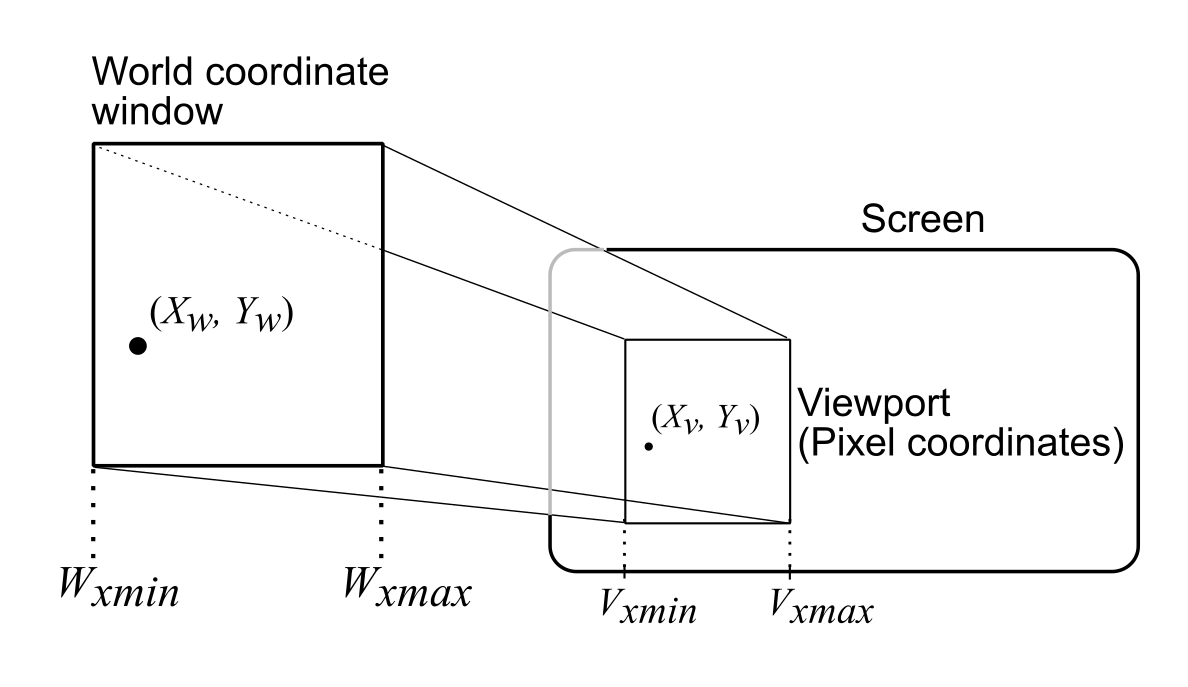
\includegraphics[scale=0.4]{normalisation}
  \centering
\end{figure}

We then perform normalisation to compute the pixel coordinates from the world coordinates, using simple ratios.
For the $x$ direction:
\[
  \frac{X_w - W_{xmin}}{W_{xmax} - W_{xmin}} = \frac{X_v - V_{xmin}}{V_{xmax} - V_{xmin}}
\]
\[
  X_v = \frac{(X_w - W_{xmin})(V_{xmax} - V_{xmin})}{W_{xmax} - W_{xmin}} + V_{xmin}
\]

With a similar expression for $y$.

From the known values, we can form a simple pair of linear equations:
\begin{align*}
  X_v &= AX_w + B \\
  Y_v &= CY_w + D
\end{align*}

If the window is moved or resized, we must re-calculate the constants $A, B, C, D$.

\subsection{Representing Planar Polygons}
Most graphical scenes and objects are built out of planar polyhedra, three-dimensional objects whose faces are all planar polygons (\textbf{faces} or \textbf{facets}).
To describe objects made of polygons, we need the \textbf{locations} of the vertices and their \textbf{topology}.

\begin{itemize}
  \item Numerical Data - 3D coordinates of vertices.
  \item Topological Data - what is connected to what.
\end{itemize}

\begin{figure}[htb!]
  \caption{Data for a polygon.}
  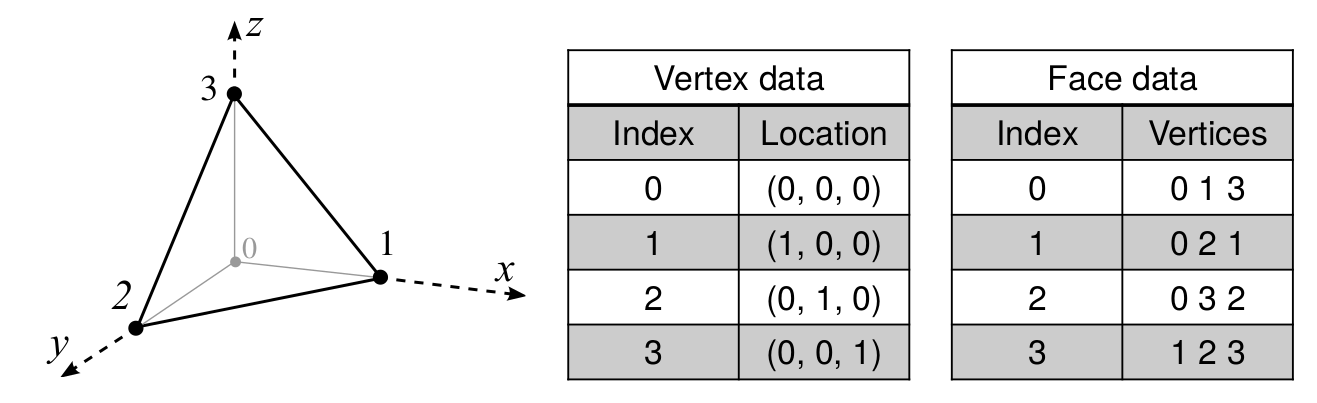
\includegraphics[scale=0.3]{polygon}
  \centering
\end{figure}

\subsection{Projections of Wire-Frame Models}
A \textbf{projection} transforms an $n$-dimensional space into an $m$-dimensional space, where $m < n$.
When projecting an object onto a surface, we first select a viewpoint then define \textit{projectors} or lines which join each vertex of the object to the viewpoint.
Where the projector intersects with the surface is defined as the projection of the corresponding vertex in the object.

The most common projections for viewing 3D scenes use a plane for the projection surface and straight lines for the projectors, these are \textbf{planar geometric projections}.
\textbf{Wire frame} models simply include points and lines, to render such a representation we need to specify only which edges join which points.
Other forms of rendering need to define the object faces.

There are two commons types of planar geometric projection:
\begin{itemize}
  \item \textbf{Parallel projection} - parallel projectors.
  \item \textbf{Perspective projection} - projectors pass through a single point (\textit{viewpoint}).
\end{itemize}

We first make some assumptions:
\begin{itemize}
  \item The viewpoint is at $z = - \infty$.
  \item The plane of projection is $z = 0$ (we can use coordinate transformations in 3D to make it so).
\end{itemize}

\subsection{Orthographic Projections}
In parallel projection, all projectors have the same direction $d$, and the viewpoint is considered to be at infinity.
For a vertex $V = (V_x, V_y, V_z)^\intercal$:
\[
  P = V + \mu d
\]

A special case is \textbf{orthographic projection}, where the projectors are perpendicular to the projection plane.
This means:
\[
  d = 
  \begin{pmatrix}
    0 \\
    0 \\
    -1
  \end{pmatrix}
\]

\begin{figure}[htb!]
  \caption{Parallel projection.}
  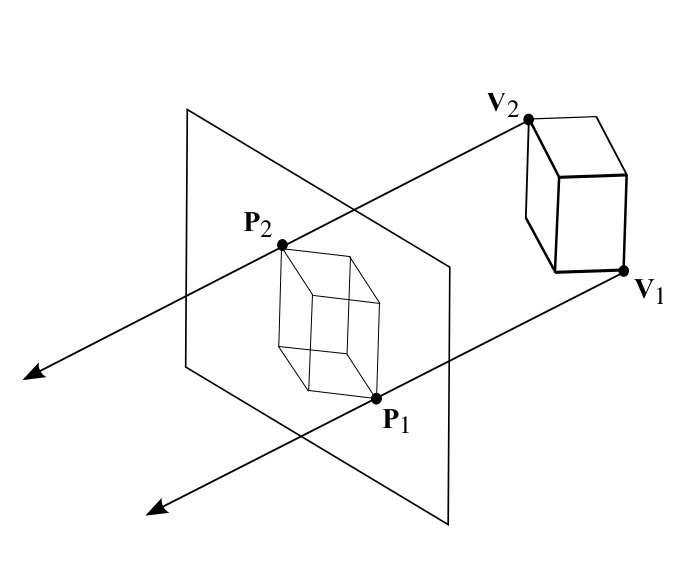
\includegraphics[scale=0.3]{parallel}
  \centering
\end{figure}

Which gives the Cartesian equations for each component:
\begin{align*}
  P_x &= V_x  & P_y &= V_y & P_z &= V_z - \mu
\end{align*}
Note that since $z = 0$, then $P_z = 0$.

This means we simply take the $x$ and $y$ coordinates:
\[
  P =
  \begin{pmatrix}
    V_x \\
    V_y \\
    0
  \end{pmatrix}
\]

\subsection{Perspective Projections}
Orthographic projections are fine in cases where we do not care about depth.
In \textbf{perspective projection}, all the projectors pass through one point in space, the \textit{centre of projection}.
If the centre of projection is on the opposite side of the plane of projection compared to the 3D object, the orientation of the image is the same as the object.
Otherwise if thecentre is between the plane and the object, the image is inverted.

\begin{figure}[htb!]
  \caption{Perspective projection where the viewpoint is on the opposite side of the object.}
  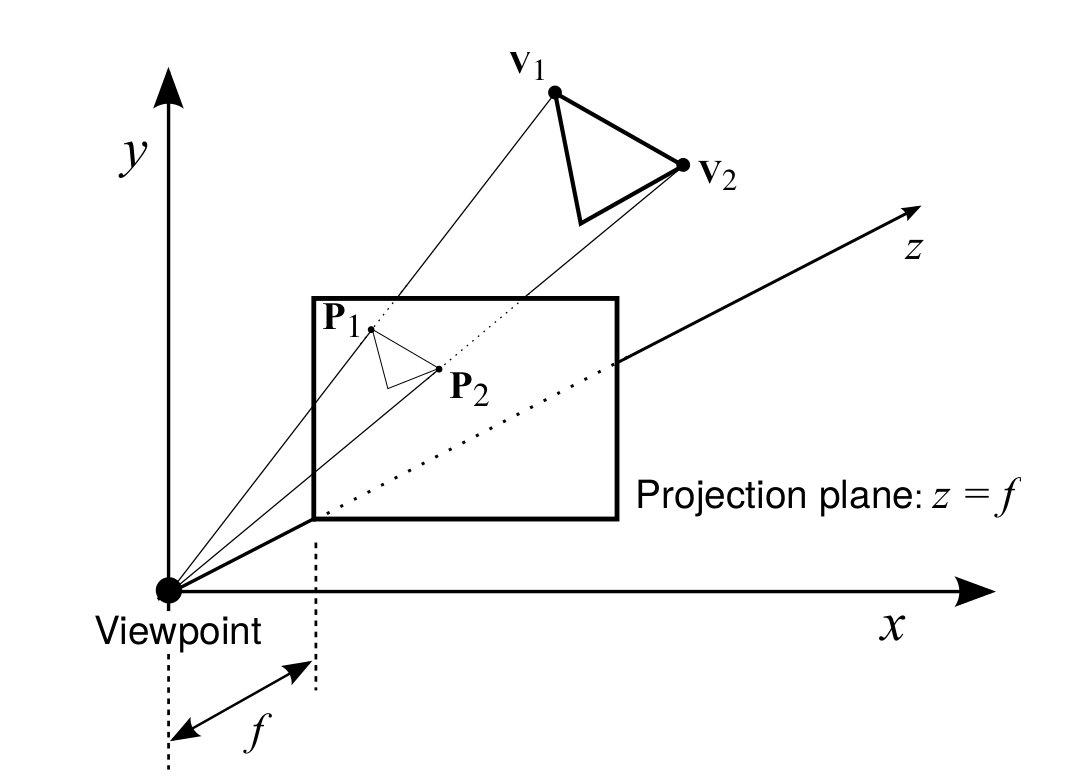
\includegraphics[scale=0.3]{perspective}
  \centering
\end{figure}

We first make two assumptions:
\begin{itemize}
  \item The centre of projection is at the origin.
  \item The projection plane is placed at a constant $z$ value, $z = f$.
\end{itemize}

The perspective projector equation from vertex $V$ is:
\[
  P = \mu V
\]

It follows that since $z = f$, then $f = \mu V_z$, and $\mu_p = f / V_z$.

This means:
\begin{align*}
  P_x = \mu_p V_x = \frac{fV_x}{V_z} && P_y = \mu_p V_y = \frac{fV_y}{V_z}
\end{align*}

We call $\mu_p$ the \textit{foreshortening} factor, if the object moves further away then $V_z$ increases and the image becomes smaller.

\subsection{Space Transformations}
Graphics scenes are defined in a particular coordinate system but we want to be able to view it at any point of our choosing.

We may also want to transform for other purposes:
\begin{itemize}
  \item Animating objects.
  \item Multiple instances.
  \item Reflections and other special effects.
\end{itemize}

In order to still be able to use canonical projection, we need to transform the coordinates of the scene so that the view direction is along the $z$-axis and the viewpoint at the origin.
That is, we want to change the coordinates of every point in the scene such that some chosen viewpoint $C$ becomes the origin, and the chosen view direction $d$ becomes the $z$-axis.
Transformation matricies can be used for nearly all simple transformations, except for translation using normal Cartesian coordinates.
We thus introduce \textbf{homogeneous coordinates}.

\subsubsection{Homogeneous Coordinates}
To express a point in homogeneous coordinates, we introduce a fourth coordinate (or \textit{ordinate}):
\[
  P =
  \begin{pmatrix}
    p_x \\
    p_y \\
    p_z \\
    s
  \end{pmatrix}
\]

The fourth ordinate is a scale factor, we use it to convert back to Cartesian form by dividing it into the other ordinates.
\[
  (p_x, p_y, p_z, s) \Leftrightarrow (\frac{p_x}{s}, \frac{p_y}{s}, \frac{p_z}{s})
\]
In most cases $s$ is $1$.

\subsubsection{Translation}
To represent translation:
\[
  \begin{pmatrix}
    1 & 0 & 0 & t_x \\
    0 & 1 & 0 & t_y \\
    0 & 0 & 1 & t_z \\
    0 & 0 & 0 & 1
  \end{pmatrix}
  \begin{pmatrix}
    p_x \\
    p_y \\
    p_z \\
    1
  \end{pmatrix}
  =
  \begin{pmatrix}
    p_x + t_x \\
    p_y + t_y \\
    p_z + t_z \\
    1
  \end{pmatrix}
\]

The inverse is:
\[
  \begin{pmatrix}
    1 & 0 & 0 & -t_x \\
    0 & 1 & 0 & -t_y \\
    0 & 0 & 1 & -t_z \\
    0 & 0 & 0 & 1
  \end{pmatrix}
\]

\subsubsection{Scaling}
To represent scaling:
\[
  \begin{pmatrix}
    s_x & 0 & 0 & 0 \\
    0 & s_y & 0 & 0 \\
    0 & 0 & s_z & 0 \\
    0 & 0 & 0 & 1
  \end{pmatrix}
  \begin{pmatrix}
    p_x \\
    p_y \\
    p_z \\
    1
  \end{pmatrix}
  =
  \begin{pmatrix}
    s_xp_x \\
    s_yp_y \\
    s_zp_z \\
    1
  \end{pmatrix}
\]

The inverse is:
\[
  \begin{pmatrix}
    1/s_x & 0 & 0 & 0 \\
    0 & 1/s_y & 0 & 0 \\
    0 & 0 & 1/s_z & 0 \\
    0 & 0 & 0 & 1
  \end{pmatrix}
\]


\subsubsection{Combining Transformations}
To combine transformations, we can multiply out their matrices and apply the transformation with the resultant matrix.

\begin{figure}[htb!]
  \caption{Importance of the order of transformations.}
  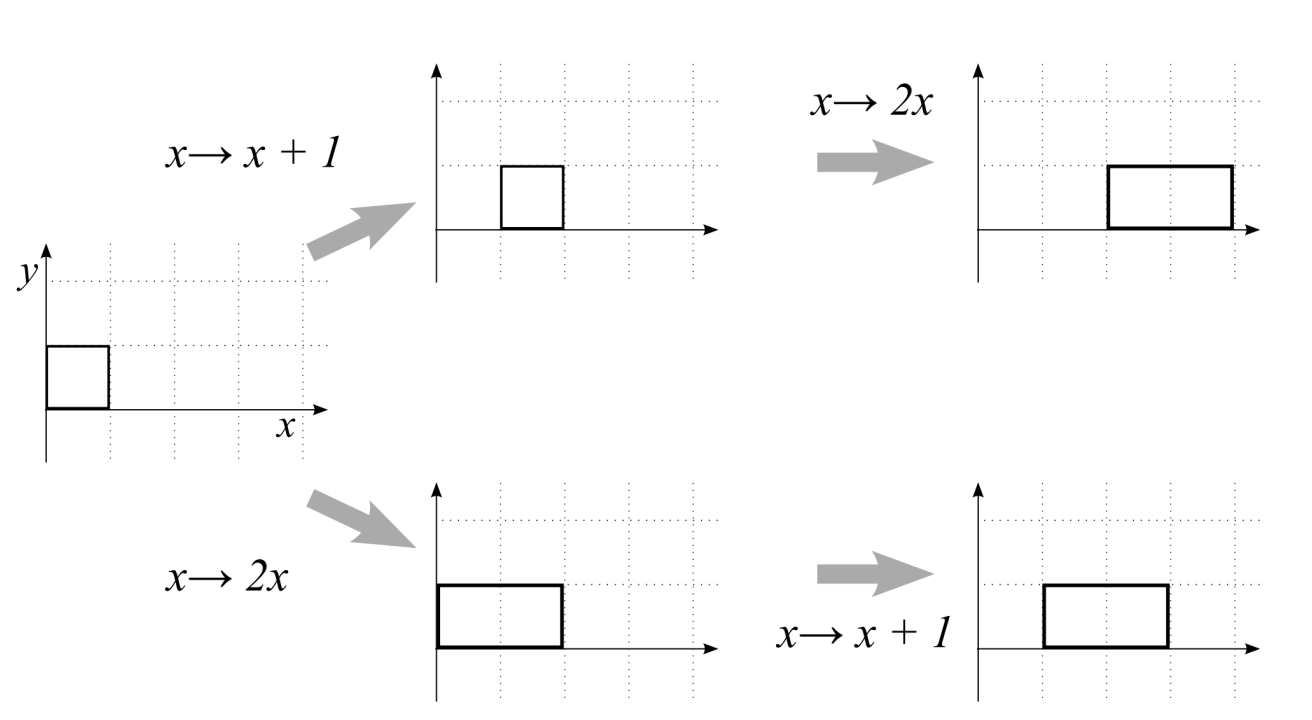
\includegraphics[scale=0.2]{combining}
  \centering
\end{figure}

Transformations are not necessarily commutative, it is important that they are carried out in the correct order.

\subsubsection{Rotation}
To define rotation we need an axis and an angle.
Matrices for rotation around the three cartesian axes are:
\begin{align*}
  \mathcal{R}_x &=
  \begin{pmatrix}
    1 & 0 & 0 & 0 \\
    0 & \cos \theta & -\sin \theta & 0 \\
    0 & \sin \theta & \cos \theta & 0 \\
    0 & 0 & 0 & 1
  \end{pmatrix} \\
  \mathcal{R}_y &=
  \begin{pmatrix}
    \cos \theta & 0 & \sin \theta & 0 \\
    0 & 1 & 0 & 0 \\
    -\sin \theta & 0 & \cos \theta & 0 \\
    0 & 0 & 0 & 1
  \end{pmatrix} \\
  \mathcal{R}_z &=
  \begin{pmatrix}
    \cos \theta &  -\sin \theta & 0 & 0 \\
    \sin \theta & \cos \theta & 0 & 0 \\
    0 & 0 & 1 & 0 \\
    0 & 0 & 0 & 1
  \end{pmatrix}
\end{align*}

\begin{figure}[htb!]
  \caption{Rotation of a coordinate ($z$-axis goes into the page).}
  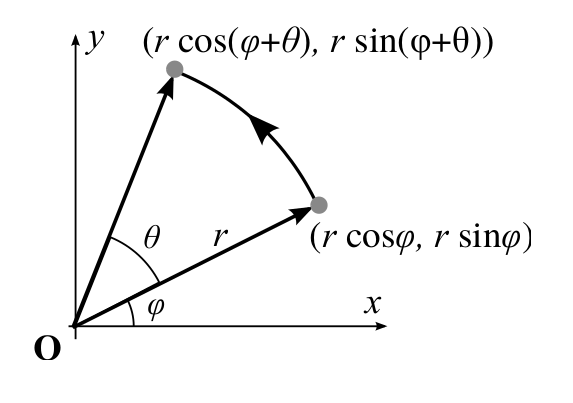
\includegraphics[scale=0.3]{deriverotate}
  \centering
\end{figure}

An example for how we derive $\mathcal{R}_z$ is as follows:
\[
  \begin{pmatrix}
    x \\
    y
  \end{pmatrix}
  =
  \begin{pmatrix}
    r \cos \varphi \\
    r \sin \varphi
  \end{pmatrix}
\]
\begin{align*}
  \begin{pmatrix}
    r \cos (\varphi + \theta) \\
    r \sin (\varphi + \theta)
  \end{pmatrix}
  &=
  \begin{pmatrix}
    r \cos \varphi \cos \theta - r \sin \varphi \sin \theta \\
    r \cos \varphi \sin \theta + r \sin \varphi \cos \theta
  \end{pmatrix} \\
  &=
  \begin{pmatrix}
    x \cos \theta - y \sin \theta \\
    x \sin \theta + y \cos \theta
  \end{pmatrix} \\
  &=
  \begin{pmatrix}
    \cos \theta & - \sin \theta \\
    \sin \theta & \cos \theta
  \end{pmatrix}
  \begin{pmatrix}
    x \\
    y
  \end{pmatrix}
\end{align*}

The $2 \times 2$ matrix is the same as the upper left corner of the matrix $\mathcal{R}_z$.

This assumes a left had axis system.
\begin{itemize}
  \item Rotation is \textbf{anti-clockwise} when looking along the axis of rotation.
  \item Rotation is \textbf{clockwise} when looking back towards the origin from the positive side of the axis.
\end{itemize}

To invert rotation, we rotate through an angle of $- \theta$, and note the follow relations:
\begin{align*}
  \cos(-\theta) &= \cos(\theta) & \sin(-\theta)=-\sin(\theta)
\end{align*}

Then for example:
\[
  \mathcal{R}_z(-\theta) = 
  \begin{pmatrix}
    \cos \theta & \sin \theta & 0 & 0 \\
    - \sin \theta & \cos \theta & 0 & 0 \\
    0 & 0 & 1 & 0 \\
    0 & 0 & 0 & 1
  \end{pmatrix}
\]

\section{Transformations for Animation}
In a viewer-centred application, we wish to view the scene from a moving position.
When the viewpoint changes, we need to transform all the coordinates of the scene.

\subsection{Flying Sequences}
Each moved viewpoint is a change of origin:
\begin{itemize}
  \item Let the required viewpoint be $C = (C_x, C_y, C_z)$.
  \item Let the required direction be $d = \begin{pmatrix} d_x \\ d_y \\ d_z \end{pmatrix}$.
\end{itemize}

The required transformation is split into three parts:
\begin{enumerate}
  \item Translation of the origin.
  \item Rotation about the $y$-axis.
  \item Rotation about the $x$-axis.
\end{enumerate}

\subsubsection{Translation of the Origin}

\begin{figure}[htb!]
  \caption{Translation of the origin.}
  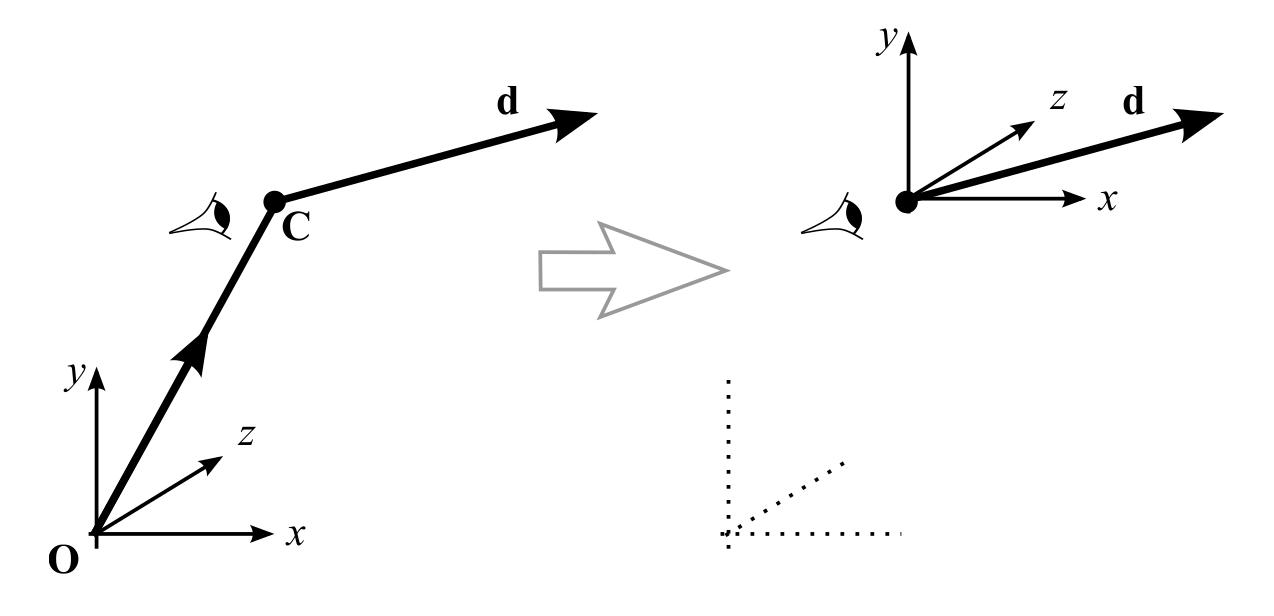
\includegraphics[scale=0.2]{transorigin}
  \centering
\end{figure}

We apply the transformation matrix:
\[
  \mathcal{A} =
  \begin{pmatrix}
    1 & 0 & 0 & -C_x \\
    0 & 1 & 0 & -C_y \\
    0 & 0 & 1 & -C_z \\
    0 & 0 & 0 & 1
  \end{pmatrix}
\]

\subsubsection{Rotation about the $y$-axis}
\begin{figure}[htb!]
  \caption{Rotation about the $y$-axis.}
  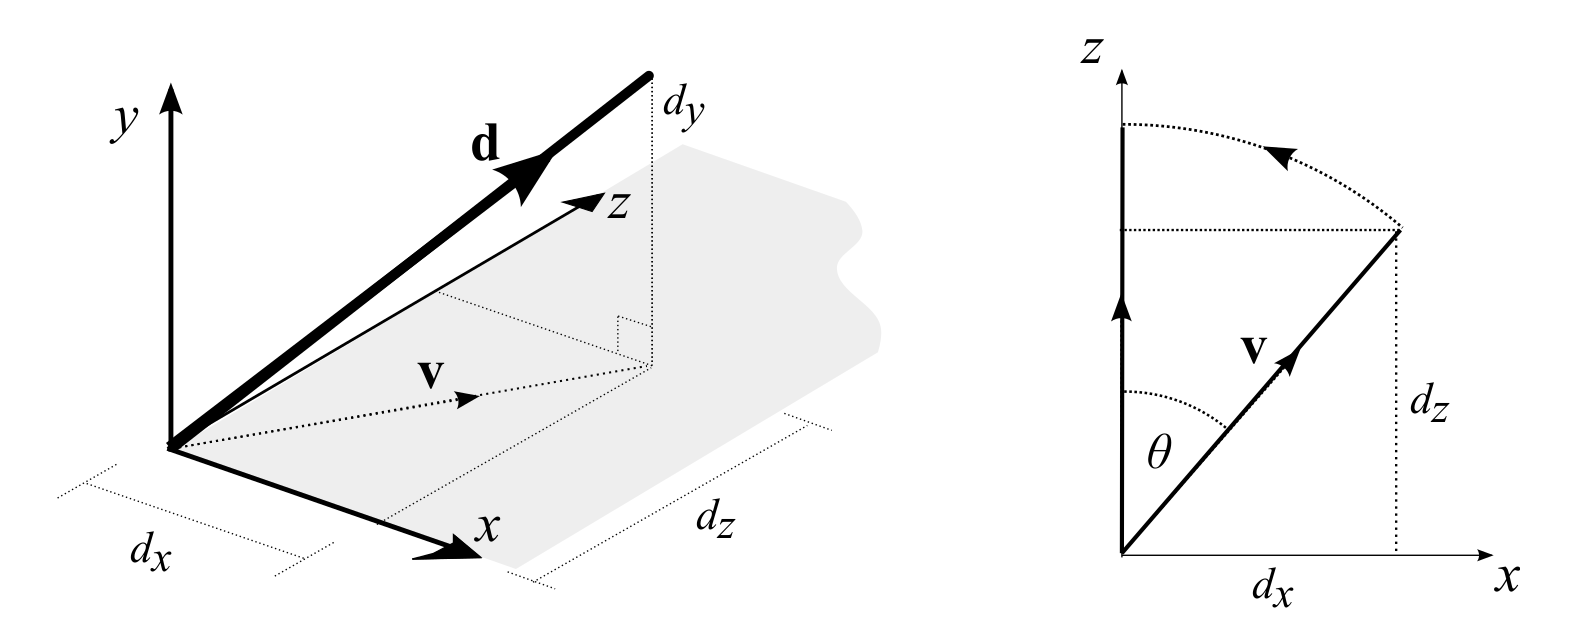
\includegraphics[scale=0.2]{roty}
  \centering
\end{figure}

We rotate about $y$ until $d$ is in the $y-z$ plane ($x = 0$):
\begin{align*}
  \lVert \textbf{v} \lVert = v = \sqrt{d_x^2 + d_z^2} && \cos \theta = d_z / v && \sin \theta = d_x / v
\end{align*}

\[
  \mathcal{B} =
  \begin{pmatrix}
    \cos \theta & 0 & -\sin \theta & 0 \\
    0 & 1 & 0 & 0 \\
    \sin \theta & 0 & \cos \theta & 0 \\
    0 & 0 & 0 & 1
  \end{pmatrix}
  =
  \begin{pmatrix}
    d_z / v & 0 & -d_x / v & 0 \\
    0 & 1 & 0 & 0 \\
    d_x / v & 0 & d_z / v & 0 \\
    0 & 0 & 0 & 1
  \end{pmatrix}
\]

\subsubsection{Rotation about the $x$-axis}
\begin{figure}[htb!]
  \caption{Rotation about the $x$-axis.}
  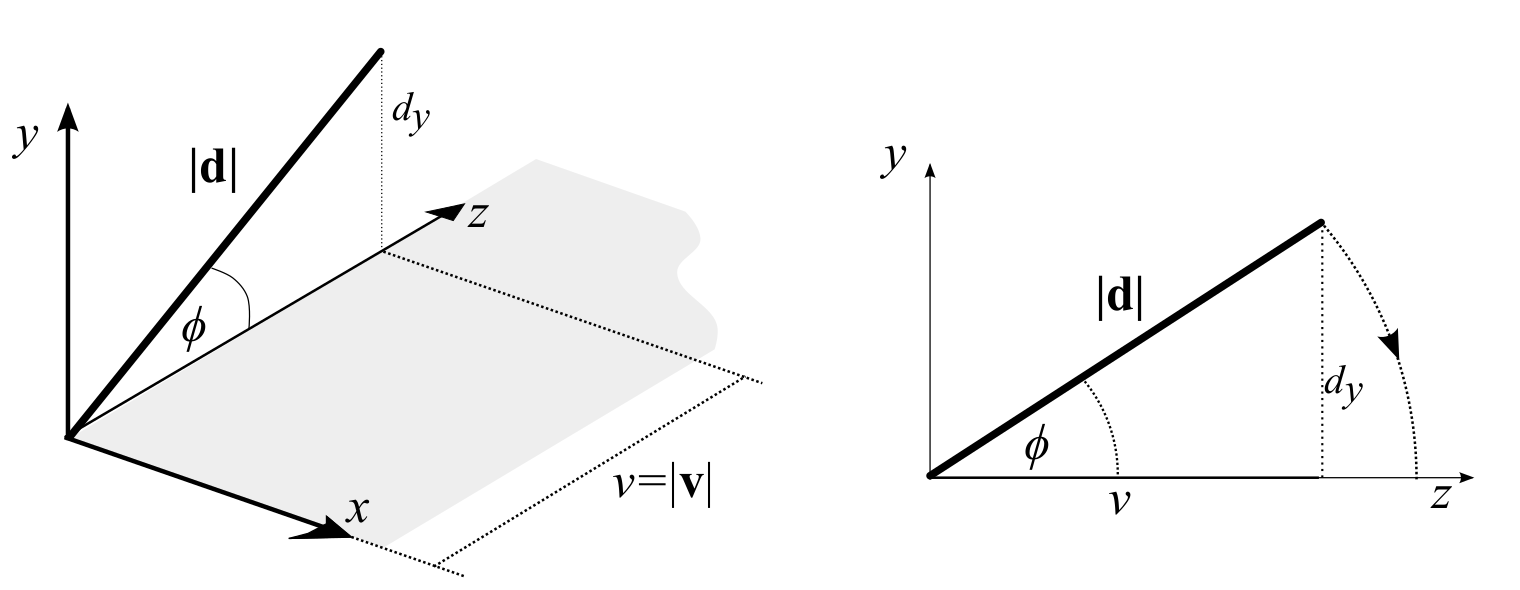
\includegraphics[scale=0.2]{rotx}
  \centering
\end{figure}

We then rotate about $x$ until $d$ points along the $z$-axis:
\begin{align*}
  v = \sqrt{d_x^2 + d_z^2} && \cos \phi = v / \lvert d \rvert && \sin \phi = d_y / \lvert d \rvert
\end{align*}

\[
  \mathcal{C} =
  \begin{pmatrix}
    1 & 0 & 0 & 0 \\
    0 & \cos \phi & -\sin \phi & 0 \\
    0 & \sin \phi & \cos \phi & 0 \\
    0 & 0 & 0 & 1
  \end{pmatrix}
  =
  \begin{pmatrix}
    1 & 0 & 0 & 0 \\
    0 & v / \lvert d \rvert & -d_y / \lvert d \rvert & 0 \\
    0 & d_y / \lvert d \rvert & v / \lvert d \rvert & 0 \\
    0 & 0 & 0 & 1
  \end{pmatrix}
\]

\subsubsection{Combining the Matrices}
\[
  \mathcal{T} = \mathcal{CBA}  
\]
Then for every point $\textbf{P}$ in the scene, we calculate:
\[
  \textbf{P}_t = \mathcal{T}\textbf{P}  
\]
The view is now in canonical form, and we can apply the standard perspective or othographic projection.

\subsubsection{Verticals}
\begin{figure}[htb!]
  \caption{Order of rotation affecting inversion.}
  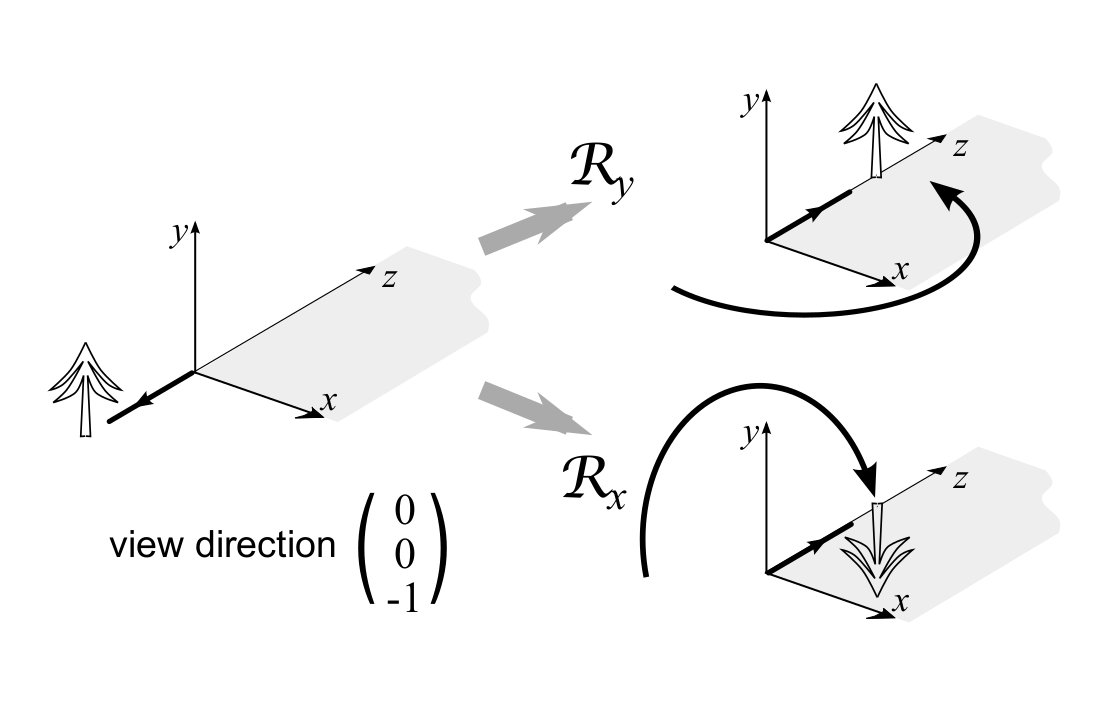
\includegraphics[scale=0.2]{invert}
  \centering
\end{figure}

Usually the $y$ direction is treated as vertical, by doing the $R_y$ transformation first, things will work out correctly.

However if we do the $R_x$ first, we could end up inverting the vertical.

\subsection{Rotation about a General Line}
To perform this transformation, we:
\begin{enumerate}
  \item Make the line of rotation one of the Cartesian axes.
  \item Rotate about the chosen axis.
  \item \textbf{Restore} the line to its original place.
\end{enumerate}

We achieve the first part through the same method as for \textit{flying sequences}: $\mathcal{CBA}$.

We then rotate about the $z$-axis, which is aligned with the general line.

Finally, we invert the initial matrices.

\[
  \mathcal{T} = \mathcal{A}^{-1} \mathcal{B}^{-1} \mathcal{C}^{-1} \mathcal{R}_z \mathcal{CBA}  
\]

\subsubsection{Other Effects}
Similar effects can be created using this approach.
\begin{eg}
  To make an object shrink (and stay in place):
  \begin{enumerate}
    \item Move the object to the origin.
    \item Apply a scaling matrix.
    \item Restore (move) the object to its place.
  \end{enumerate}
\end{eg}

\subsection{Projection by Matrix Multiplication}
\subsection{Orthographic Projection Matrix}
\[
  \mathcal{M}_o =
  \begin{pmatrix}
    1 & 0 & 0 & 0 \\
    0 & 1 & 0 & 0 \\
    0 & 0 & 0 & 0 \\
    0 & 0 & 0 & 1
  \end{pmatrix}
\]
\[
  \mathcal{M}_o
  \begin{pmatrix}
    x \\ y \\ z \\ 1
  \end{pmatrix}
  =
  \begin{pmatrix}
    x \\ y \\ 0 \\ 1
  \end{pmatrix}
\]

\subsection{Perspective Projection Matrix}
\[
  \mathcal{M}_p =
  \begin{pmatrix}
    1 & 0 & 0 & 0 \\
    0 & 1 & 0 & 0 \\
    0 & 0 & 1 & 0 \\
    0 & 0 & 1 / f & 0
  \end{pmatrix}
\]
\[
  \mathcal{M}_p
  \begin{pmatrix}
    x \\ y \\ z \\ 1
  \end{pmatrix}
  =
  \begin{pmatrix}
    x \\ y \\ z \\ z / f
  \end{pmatrix}
\]

We then normalise the result to get:
\[
  \begin{pmatrix} xf/z \\ yf/z \\ f \\ 1 \end{pmatrix}  
\]
as required.

\subsection{Singular}
Both projection matricies are singular, notice each has a column of zeroes.
This means they cannot be inverted: we cannot reconstruct the original 3D scene from a 2D image.

\subsection{Homogeneous Coordinates and Vectors}
\begin{itemize}
  \item \textbf{Position vectors} - $\begin{pmatrix} x \\ y \\ z \\ s \end{pmatrix}$.
    \begin{itemize}
      \item Non-zero final ordinate ($s$).
      \item Can be normalised into Cartesian form.
      \item \textit{Fixed point in space.}
    \end{itemize}
  \item \textbf{Direction vectors} - $\begin{pmatrix} x \\ y \\ z \\ 0 \end{pmatrix}$.
    \begin{itemize}
      \item Zero final ordinate.
      \item Have direction and magnitude.
      \item \textit{Not associated with a particular point.}
    \end{itemize}
\end{itemize}

\subsubsection{Addition of Vectors}
Adding \textbf{two direction vectors} results in a direction vector (notice the zero final ordinate):
\[
  \begin{pmatrix} x_i \\ y_i \\ z_i \\ 0 \end{pmatrix} 
  +
  \begin{pmatrix} x_j \\ y_j \\ z_j \\ 0 \end{pmatrix} 
  =
  \begin{pmatrix} x_i + x_j \\ y_i + y_j \\ z_i + z_j \\ 0 \end{pmatrix} 
\]

Adding a \textbf{direction vector to a position vector} results in a position vector:
\[
  \begin{pmatrix} X \\ Y \\ Z \\ 1 \end{pmatrix} 
  +
  \begin{pmatrix} x \\ y \\ z \\ 0 \end{pmatrix} 
  =
  \begin{pmatrix} X + x \\ Y + y \\ Z + z \\ 1 \end{pmatrix} 
\]

Adding \textbf{two position vectors} results in their mid-point:
\[
  \begin{pmatrix} X_a \\ Y_a \\ Z_a \\ 1 \end{pmatrix} 
  +
  \begin{pmatrix} X_b \\ Y_b \\ Z_b \\ 1 \end{pmatrix} 
  =
  \begin{pmatrix} X_a + X_b \\ Y_a + Y_b \\ Z_a + Z_b \\ 2 \end{pmatrix} 
  =
  \begin{pmatrix} (X_a + X_b) / 2 \\ (Y_a + Y_b) / 2 \\ (Z_a + Z_b) / 2 \\ 1 \end{pmatrix} 
\]

\subsection{Transformation Matrices}
\subsubsection{Structure}
\[
  \begin{pmatrix}
    q_x & r_x & s_x & C_x \\
    q_y & r_y & s_y & C_y \\
    q_z & r_z & s_z & C_z \\
    0 & 0 & 0 & 1
  \end{pmatrix}
\]
\begin{itemize}
  \item The bottom row is always $\begin{matrix}0&0&0&1\end{matrix}$.
  \item The columns comprise of three direction vectors and one position vector.
\end{itemize}

\subsubsection{Characteristics}
When we multiply a direction vector, the last ordinate ensures it is not affected by translation:
\[
  \begin{pmatrix}
    q_x & r_x & s_x & C_x \\
    q_y & r_y & s_y & C_y \\
    q_z & r_z & s_z & C_z \\
    0 & 0 & 0 & 1
  \end{pmatrix}
  \begin{pmatrix} * \\ * \\ * \\ 0 \end{pmatrix}
  =
  \begin{pmatrix} * \\ * \\ * \\ 0 \end{pmatrix}
\]

When we multiply a position vector, the last ordinate ensures all vectors have the same displacement:
\[
  \begin{pmatrix}
    q_x & r_x & s_x & C_x \\
    q_y & r_y & s_y & C_y \\
    q_z & r_z & s_z & C_z \\
    0 & 0 & 0 & 1
  \end{pmatrix}
  \begin{pmatrix} * \\ * \\ * \\ 1 \end{pmatrix}
  =
  \begin{pmatrix} * + C_x \\ * + C_y \\ * + C_z \\ 1 \end{pmatrix}
\]

If we do not shear the object, $q$, $r$, $s$ will remain orthogonal:
\[
  q \cdot r = r \cdot s = q \cdot s = 0  
\]

\subsubsection{Meaning of the Individual Columns}
When we multiply the matrix by unit vectors, we get the individual columns of the matrix:
\[
  \begin{pmatrix}
    q_x & r_x & s_x & C_x \\
    q_y & r_y & s_y & C_y \\
    q_z & r_z & s_z & C_z \\
    0 & 0 & 0 & 1
  \end{pmatrix}
  \begin{pmatrix} 1 & 0 & 0 & 0 \end{pmatrix}
  =
  \begin{pmatrix} q_x & q_y & q_z & 0 \end{pmatrix}
\]

This means that the columns are the original axis system after transforming to the new coordinate system:
\begin{itemize}
  \item \textbf{q} is the transformed $x$-axis.
  \item \textbf{r} is the transformed $y$-axis.
  \item \textbf{s} is the transformed $z$-axis.
  \item \textbf{C} is the transformed origin.
\end{itemize}

\subsubsection{Effect of a Transformation Matrix}
\begin{figure}[htb!]
  \caption{Effect of a transformation matrix.}
  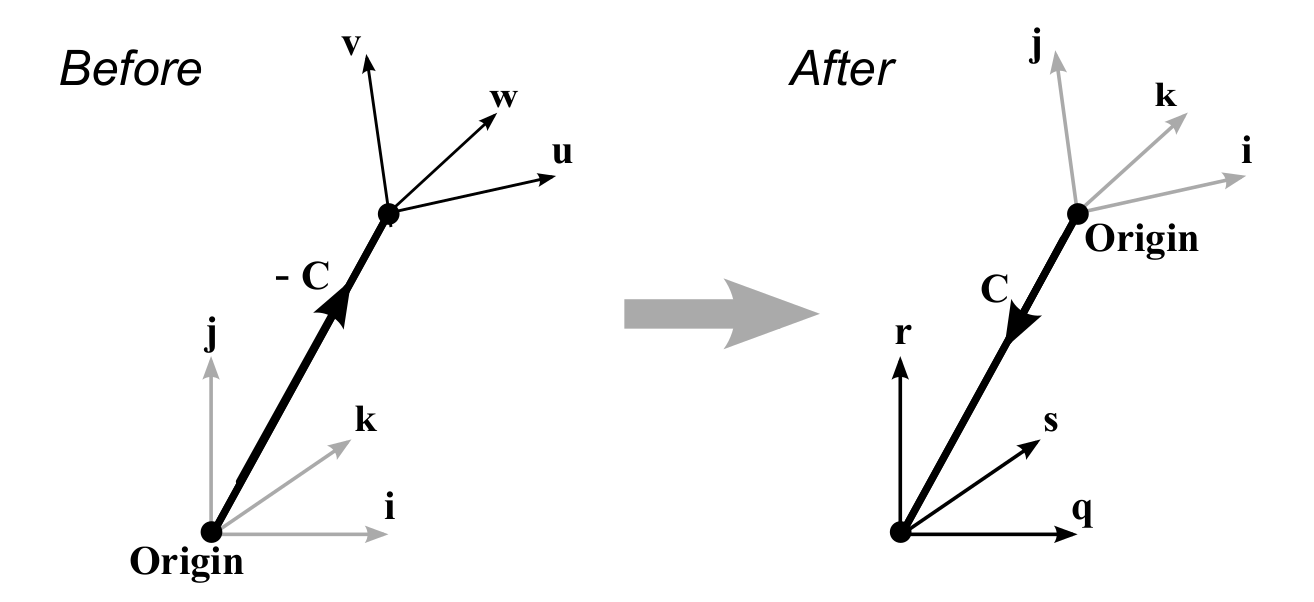
\includegraphics[scale=0.2]{effecttransform}
  \centering
\end{figure}

We get the old axes and origin in the new coordinate system:
\[
  \begin{pmatrix}
    q_x & r_x & s_x & C_x \\
    q_y & r_y & s_y & C_y \\
    q_z & r_z & s_z & C_z \\
    0 & 0 & 0 & 1
  \end{pmatrix}
  =
  \begin{bmatrix} \textbf{q} & \textbf{r} & \textbf{s} & \textbf{C} \end{bmatrix}
\]

\subsection{General Viewing Matrix Transformation}
Normally, we are not given the transformation matrix, but the view direction $\textbf{d}$ and location $\textbf{C}$ instead.

\subsubsection{Dot Product}
\begin{defn}
  The \textbf{dot product} is defined:
  \[
    P \cdot u = \lvert P \rvert \lvert u \rvert \cos \theta  
  \]
\end{defn}

\begin{figure}[htb!]
  \caption{The dot product as an ordinate of $P$.}
  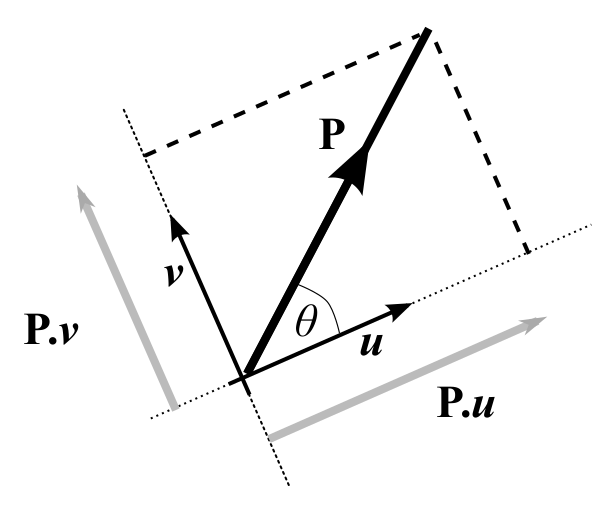
\includegraphics[scale=0.2]{dotproduct}
  \centering
\end{figure}

\begin{itemize}
  \item If $u$ is a unit vector, then $P \cdot u = \lvert P \rvert \cos \theta$.
  \item If $u$ is along a coordinate axis, then $P \cdot u$ is the ordinate of $P$ in the direction of $u$.
\end{itemize}

\subsubsection{Changing Axes by Projection}
\begin{figure}[htb!]
  \caption{Transforming a point $\textbf{P}$ to a different axes.}
  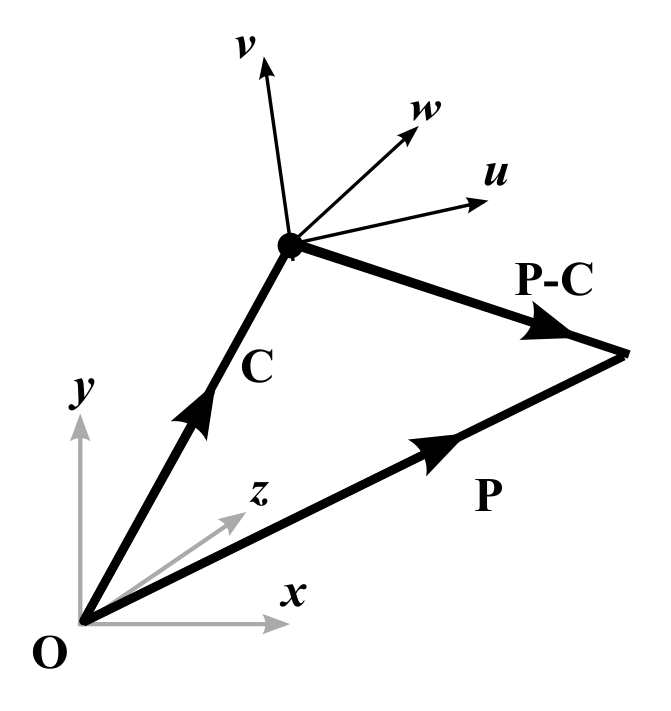
\includegraphics[scale=0.2]{changingaxes}
  \centering
\end{figure}

We can express projections using the dot product:
\begin{alignat*}{2}
  P_x^t &= (\textbf{P} - \textbf{C}) \cdot \textbf{u} &&= \textbf{P} \cdot \textbf{u} - \textbf{C} \cdot \textbf{u} \\
  P_y^t &= (\textbf{P} - \textbf{C}) \cdot \textbf{v} &&= \textbf{P} \cdot \textbf{v} - \textbf{C} \cdot \textbf{v} \\
  P_z^t &= (\textbf{P} - \textbf{C}) \cdot \textbf{w} &&= \textbf{P} \cdot \textbf{w} - \textbf{C} \cdot \textbf{w}
\end{alignat*}

In matrix notation:
\[
  \begin{pmatrix} P_x^t \\ P_y^t \\ P_z^t \\ 1 \end{pmatrix}
  =
  \begin{pmatrix}
    u_x & u_y & u_z & -\textbf{C} \cdot \textbf{u} \\ 
    v_x & v_y & v_z & -\textbf{C} \cdot \textbf{v} \\ 
    w_x & w_y & w_z & -\textbf{C} \cdot \textbf{w} \\ 
    0 & 0 & 0 & 1
  \end{pmatrix}
  \begin{pmatrix} P_x \\ P_y \\ P_z \\ 1 \end{pmatrix}
\]

By maintaining values of $\textbf{C}, \textbf{u}, \textbf{v}, \textbf{w}$ throughout an animation sequence, we can write down the correct scene transformation matrix.

\subsubsection{Returning to Flying Sequences}
As we know $\textbf{d}$ is the direction of the new axis, then
\[
  \textbf{w} = \frac{\textbf{d}}{\lvert \textbf{d} \rvert}
\]

We can write $\textbf{u}$ in terms of some vector $\textbf{p}$ in the horizontal direction:
\[
  \textbf{u} = \frac{\textbf{p}}{\lvert \textbf{p} \rvert}
\]
and set $p_y = 0$ to ensure it has no vertical component.

We can write $\textbf{v}$ in terms of some vector $\textbf{q}$ in the vertical direction:
\[
  \textbf{v} = \frac{\textbf{q}}{\lvert \textbf{q} \rvert}
\]
and force $q_y = 1$ to ensure it has a positive $y$ component.

We now have:
\begin{align*}
  \textbf{p} &= \begin{pmatrix} p_x \\ 0 \\ p_z \end{pmatrix}
  & \textbf{q} &= \begin{pmatrix} q_x \\ 1 \\ q_z \end{pmatrix}
\end{align*}

It must be that:
\[
  \textbf{d} = \textbf{p} \times \textbf{q} 
\]
since $\textbf{d}$ is orthogonal to both, and the magnitude of the new vectors has not been set.

Evaluating the cross products results in:
\begin{align*}
  d_x &= -p_z \\
  d_y &= p_zq_x - p_xq_z \\
  d_z &= p_x
\end{align*}

Which means:
\[
  \textbf{p} = \begin{pmatrix} d_z \\ 0 \\ -d_x \end{pmatrix} 
\]

Using the dot product with $\textbf{p}$ and $\textbf{q}$, then:
\[
  \textbf{p} \cdot \textbf{q} = p_xq_x + p_zq_z = 0
\]
which we solve with the result from the cross product:
\[
  d_y = p_zq_x - p_xq_z
\]

Once we have expressions for $\textbf{p}$ and $\textbf{q}$ in terms of given vector $\textbf{d}$, then we have obtained:
\begin{align*}
  \textbf{u} &= \frac{\textbf{p}}{\lvert \textbf{p} \rvert} &
  \textbf{v} &= \frac{\textbf{q}}{\lvert \textbf{q} \rvert} &
  \textbf{w} &= \frac{\textbf{d}}{\lvert \textbf{d} \rvert}
\end{align*}
which we use to write down:
\[
  \begin{pmatrix}
    u_x & u_y & u_z & -\textbf{C} \cdot \textbf{u} \\ 
    v_x & v_y & v_z & -\textbf{C} \cdot \textbf{v} \\ 
    w_x & w_y & w_z & -\textbf{C} \cdot \textbf{w} \\ 
    0 & 0 & 0 & 1
  \end{pmatrix}
\]

\section{Clipping}
\begin{defn}
  \textbf{Clipping} is the process of eliminating portions of objects outside the viewing frustum to avoid degeneracy and improve efficiency.
\end{defn}

\begin{figure}[htb!]
  \caption{The view frustum.}
  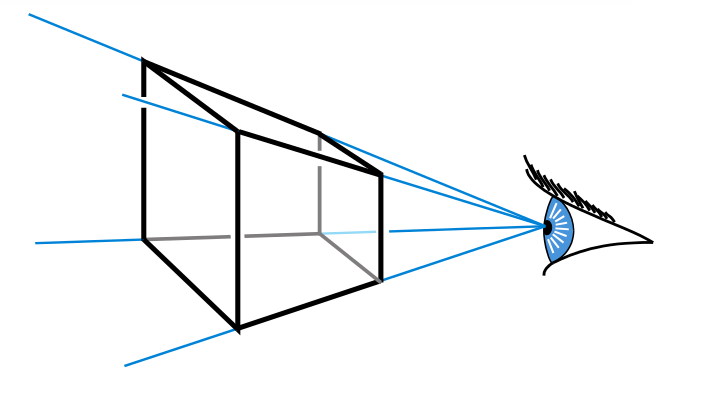
\includegraphics[scale=0.3]{frustum}
  \centering
\end{figure}

The view frustum is the boundaries of the image plane projected in 3D, consisting of a near and far clipping plane, with additional user defined clipping planes.

When do we clip?
\begin{itemize}
  \item Before perspective transform in 3D space (natural).
  \item In homogeneous coordinates after perspective transform (simple).
  \item In the transformed 3D screen space after perspective division (messy).
\end{itemize}

\subsection{Halfspace}
\begin{figure}[htb!]
  \caption{The concept of a halfspace.}
  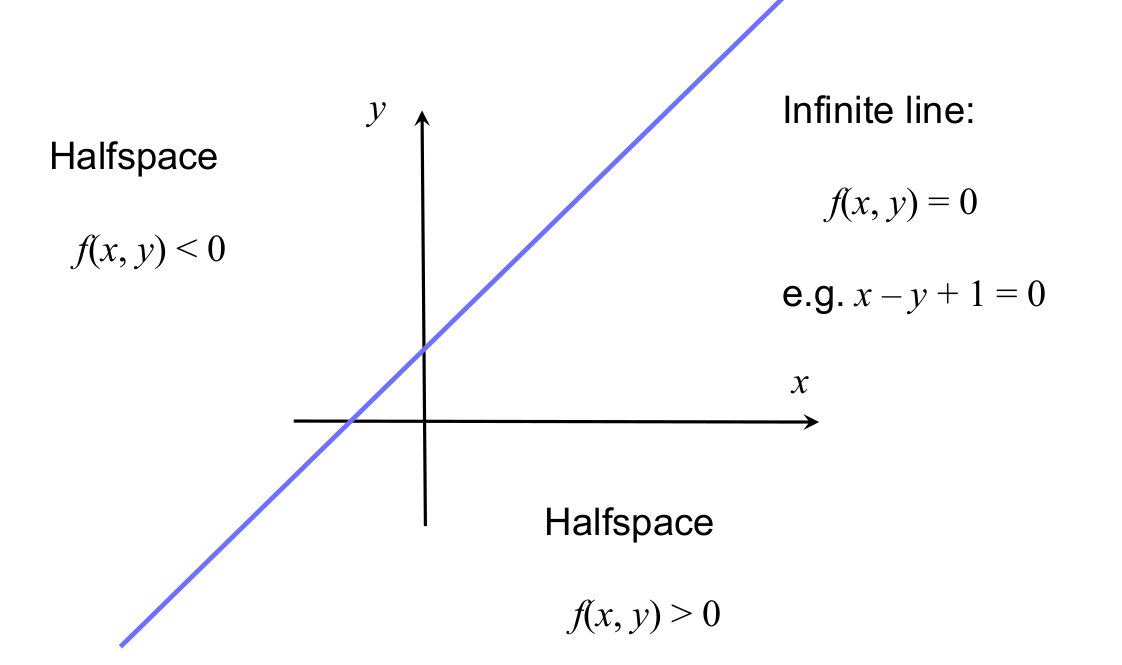
\includegraphics[scale=0.3]{halfspace}
  \centering
\end{figure}
We can use halfspaces to perform a test on all the points in the scene, to determine if they should be discarded or drawn.

In planes, we use the general equations:
\[
  f(x, y, z) = 0 \text{ or } Ax + By + Cz + D = 0
\]

\subsection{Homogeneous Coordinates}
We can link the plane equation to homogeneous coordinates:
\[
  \textbf{H} = \begin{pmatrix} A \\ B \\ C \\ D \end{pmatrix}  
\]
However, each point has an infinite number of equivalent homogenous coordinates as they can be scaled, $\begin{pmatrix} sx & sy & sz & sw \end{pmatrix}$.

We solve this by scaling $\textbf{H}$ so that $\begin{pmatrix} A & B & C \end{pmatrix}$ becomes normalized:
\[
  A^2 + B^2 + C^2 = 1  
\]

\begin{figure}[htb!]
  \caption{Using $\textbf{H}$ to find the distance to a point $\textbf{p}$.}
  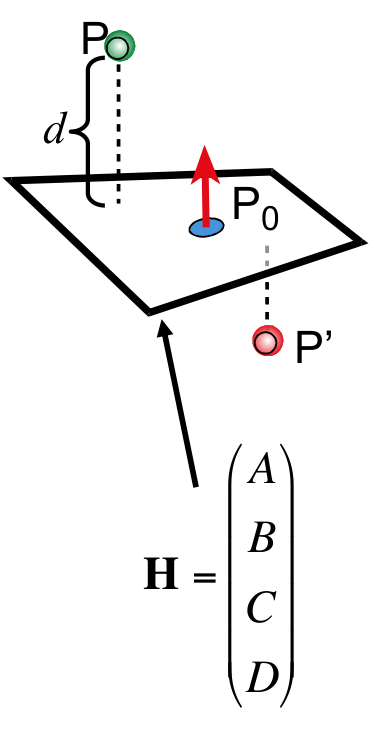
\includegraphics[scale=0.3]{signeddistance}
  \centering
\end{figure}

Then the distance is calculated:
\[
  d = \textbf{H} \cdot \textbf{p} = \textbf{H}^\intercal \textbf{p} 
\]
since $\textbf{H}$ is the normal of the plane.

$d$ is a \textbf{signed distance}:
\begin{itemize}
  \item Positive $\rightarrow$ inside the plane, pass through.
  \item Negative $\rightarrow$ outside the plane, clip (or cull or reject).
\end{itemize}

We do not actually need to normalize as we test only the sign of $\textbf{H} \cdot \textbf{p}$.

\subsection{Clipping with respect to View Frustum}
We test a point $\textbf{p}$ against each of the 6 planes, where each normal $\textbf{H}$ is oriented towards the interior.

\begin{align*}
  \textbf{H}_{near} &= \begin{pmatrix} 0 & 0 & 1 & -near \end{pmatrix}^\intercal \\
  \textbf{H}_{far} &= \begin{pmatrix} 0 & 0 & -1 & far \end{pmatrix}^\intercal \\
  \textbf{H}_{bottom} &= \begin{pmatrix} 0 &  near & -bottom & 0 \end{pmatrix}^\intercal \\
  \textbf{H}_{top} &= \begin{pmatrix} 0 & -near & top & 0 \end{pmatrix}^\intercal \\
  \textbf{H}_{left} &= \begin{pmatrix} -near  & 0 & left & 0 \end{pmatrix}^\intercal \\
  \textbf{H}_{right} &= \begin{pmatrix} near & 0 & -right & 0 \end{pmatrix}^\intercal
\end{align*}

We can derive the first two from observing the frustum and recalling that that the viewpoint looks along the $z$-axis.

The rest can be derived by taking points from the frustum corners:
\[
  \begin{pmatrix} l \\ b \\ n \end{pmatrix}
  \times
  \begin{pmatrix} b \\ b \\ n \end{pmatrix}
  =
  \begin{vmatrix}
    \hat{i} & \hat{j} & \hat{k} \\
    l & b & n \\
    r & b & n
  \end{vmatrix}
  =
  \begin{pmatrix} 0 & n & -b \end{pmatrix}
\]

\begin{alignat*}{2}
  \quad & (\textbf{P} - \textbf{P}_1) \cdot \textbf{n} &&= 0 \\
  \implies & ny - bz &&= 0 \\
  \implies & \textbf{H}_{bottom} &&= \begin{pmatrix} 0 & n & -b & 0 \end{pmatrix}^\intercal
\end{alignat*}

\subsection{Line-Plane Intersection}
Explicit (parametric) line equation:
\[
  \textbf{L}(\mu) = \textbf{p}_0 + \mu(\textbf{p}_1 - \textbf{p}_0) = \mu \textbf{p}_1 + (1 - \mu) \textbf{p}_0
\]

To compute the intersection point, we use the fact that $(\textbf{P} - \textbf{P}_1) \cdot \textbf{n} = 0$:
\begin{enumerate}
  \item Let the intersection point be $\mu \textbf{p}_1 + (1 - \mu) \textbf{p}_0$.
  \item Choose $\textbf{v}$ to be any point on the plane.
  \item A vector in the plane is given by $\mu \textbf{p}_1 + (1 - \mu) \textbf{p}_0 - \textbf{v}$.
  \item Then $\textbf{n} \cdot (\mu \textbf{p}_1 + (1 - \mu) \textbf{p}_0 - \textbf{v}) = 0$
  \item Solve for $\mu$ to find the point of intersection.
\end{enumerate}

\subsubsection{Segment Clipping}
\begin{itemize}
  \item If $\textbf{H} \cdot \textbf{p} > 0$ and $\textbf{H} \cdot \textbf{q} < 0$: clip $\textbf{q}$ to plane.
  \item If $\textbf{H} \cdot \textbf{p} < 0$ and $\textbf{H} \cdot \textbf{q} > 0$: clip $\textbf{p}$ to plane.
  \item If $\textbf{H} \cdot \textbf{p} > 0$ and $\textbf{H} \cdot \textbf{q} > 0$: pass through.
  \item If $\textbf{H} \cdot \textbf{p} < 0$ and $\textbf{H} \cdot \textbf{q} < 0$: clipped out.
\end{itemize}

\subsubsection{Clipping against the Frustum}
For each frustum plane $\textbf{H}$, we apply segment clipping.
This results in a single segment.

\subsection{Clipping and Containment}
Clipping can be carried out against any object.
We to develop a test for containment, to determine if a point is inside or outside the object, namely for convex and concave objects.

\subsubsection{Convex Objects}
Convex objects are defined by:
\begin{enumerate}
  \item A line joining any two points on the boundary lies inside the object.
  \item The object is the intersection of planar halfspaces.
\end{enumerate}
All points of the object must lie entirely to one side of each face - we use this to check if a shape is convex, and to check if a point is contained within the object.

\begin{figure}[htb!]
  \caption{Vector test for containment on a convex shape.}
  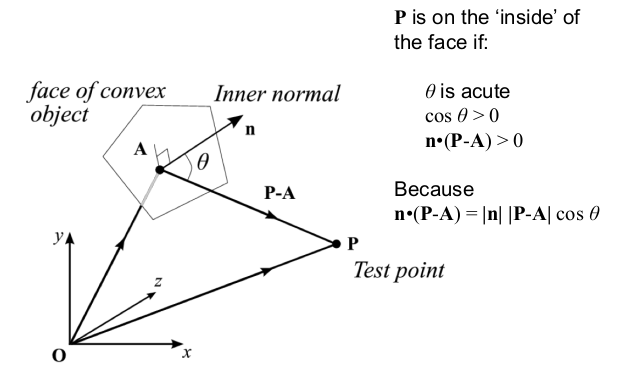
\includegraphics[scale=0.5]{containmentvector}
  \label{fig:vectortest}
  \centering
\end{figure}

The vector formulation (figure \ref{fig:vectortest}) does not require finding the plane equation of a face, but does require finding the normal vector to the plane.
This involves finding the cross product of two vectors on the plane, say two edge vectors.

\begin{figure}[htb!]
  \caption{Finding a normal vector using two edge vectors.}
  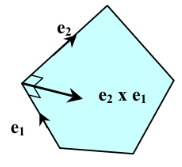
\includegraphics[scale=0.5]{edgenormal}
  \centering
\end{figure}

Care must be taken to ensure the normal found is an \textbf{inner normal}, see figure \ref{fig:innernormalcheck}.

\begin{figure}[htb!]
  \caption{Finding a normal vector using two edge vectors.}
  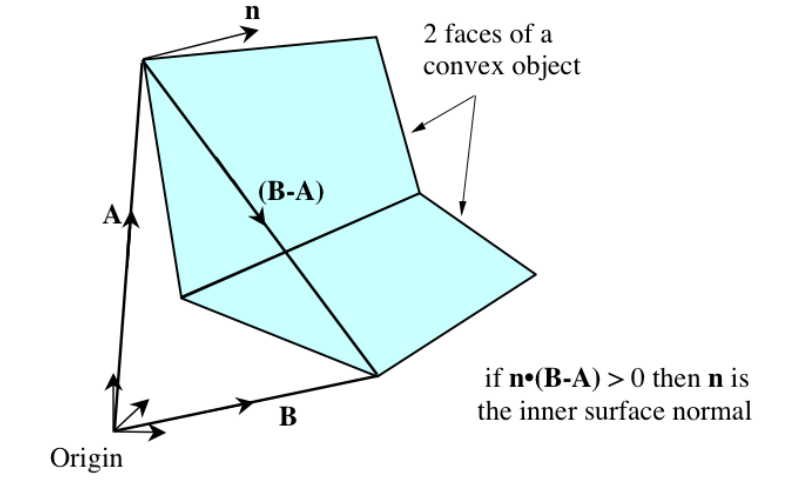
\includegraphics[scale=0.4]{innernormal}
  \label{fig:innernormalcheck}
  \centering
\end{figure}

\section{Graphics Pipeline}

\begin{figure}[htb!]
  \caption{The graphics pipeline.}
  \centering
  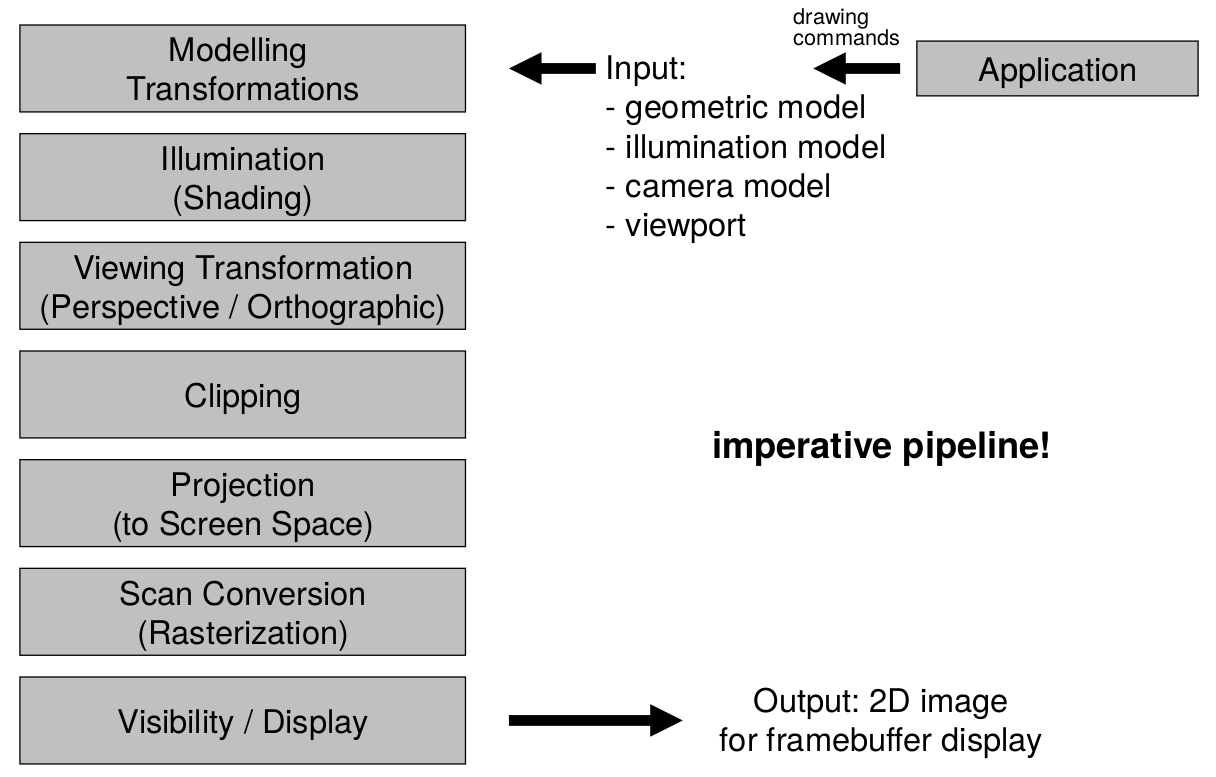
\includegraphics[scale=0.3]{pipeline}
\end{figure}

\begin{itemize}
  \item \textbf{Modelling Transformations}:
    \begin{itemize}
      \item 3D models are defined in their own coordinate system.
      \item These models are oriented within the common (world) coordinate frame.
    \end{itemize}
  \item \textbf{Illumination (Shading)}:
    \begin{itemize}
      \item Vertices are lit according to material properties, surface properties, and light sources.
      \item Local lighting model used.
    \end{itemize}
  \item \textbf{Viewing Transformation (Perspective/Orthographic)}:
    \begin{itemize}
      \item World space is mapped to camera space (matrix evaluation).
      \item Viewing position is transformed to origin and viewing direction oriented along some axis (usually $z$).
    \end{itemize}
  \item \textbf{Clipping}:
    \begin{itemize}
      \item Portions of the scene outside the view frustum are removed.
      \item Transform to \textit{Normalized Device Coordinates}.
    \end{itemize}
  \item \textbf{Projection (to Screen Space)}:
    \begin{itemize}
      \item Objects projected to the 2D imaging plane.
    \end{itemize}
  \item \textbf{Rasterizaton}
    \begin{itemize}
      \item Objects rasterized to pixels.
      \item Interpolate values inside objects.
    \end{itemize}
  \item \textbf{Visibility/Display}:
    \begin{itemize}
      \item Occulsions and transparency blending.
      \item Determines which objects closest, and therefore visible.
      \item Depth buffer.
    \end{itemize}
\end{itemize}

Real-time CGI is very computationally demanding.
Therefore we use specialized hardware - \textit{graphics processing units} (GPUs).
Most real-time graphics is based on rasterization of graphic primitives and implemented in hardware, controlled through an API such as \textit{OpenGL}.

\begin{defn}
  A \textbf{vertex} is a point in space defining geometry.
\end{defn}

\begin{defn}
  A \textbf{fragment} is a sample produced during rasterization; multiple fragments are merged into pixels.
\end{defn}

The pipeline is split into three main stages: application, geometry, and rasterization.

\subsection{Application Stage}
This is executed in software, so it cannot be divided into individual steps that are executed in a pipeline.

Changes are made to the scene as required, perhaps due to user interaction or in an animation.
The new scene with all its primitives is then forwarded to the next step of the pipeline.

The most important task performed is data management.
This includes acceleration techniques using spatial subdivision schemes that optimize the data currently stored in memory.
A modern day computer game's world and textures are much bigger than what could be loaded into the available RAM or graphics memory.

\subsection{Geometry Stage}
\begin{figure}[htb!]
  \centering
  \caption{The geometry stage.}
  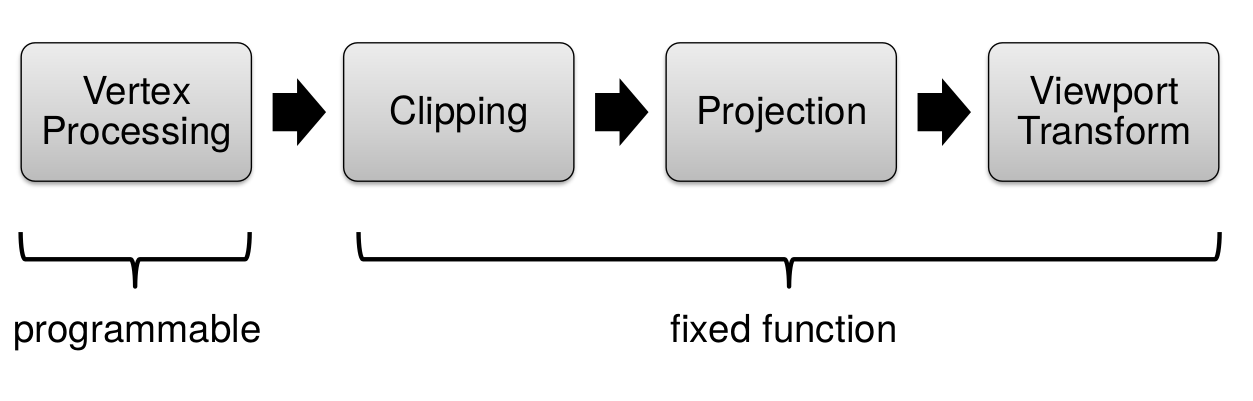
\includegraphics[scale=0.3]{geometrystage}
\end{figure}

This is responsible for the majority of operations with polygons and their vertices

\subsubsection{Vertex Processing}
The input vertex stream, composed of arbitrary vertex attributes, is transformed into a stream of vertices, composed of their clip space coordinates and additional user-define attributes, mapped onto the screen by the vertex shader.

\begin{figure}[htb!]
  \centering
  \caption{Possible pre-combinations of transformation matrices and their common names.}
  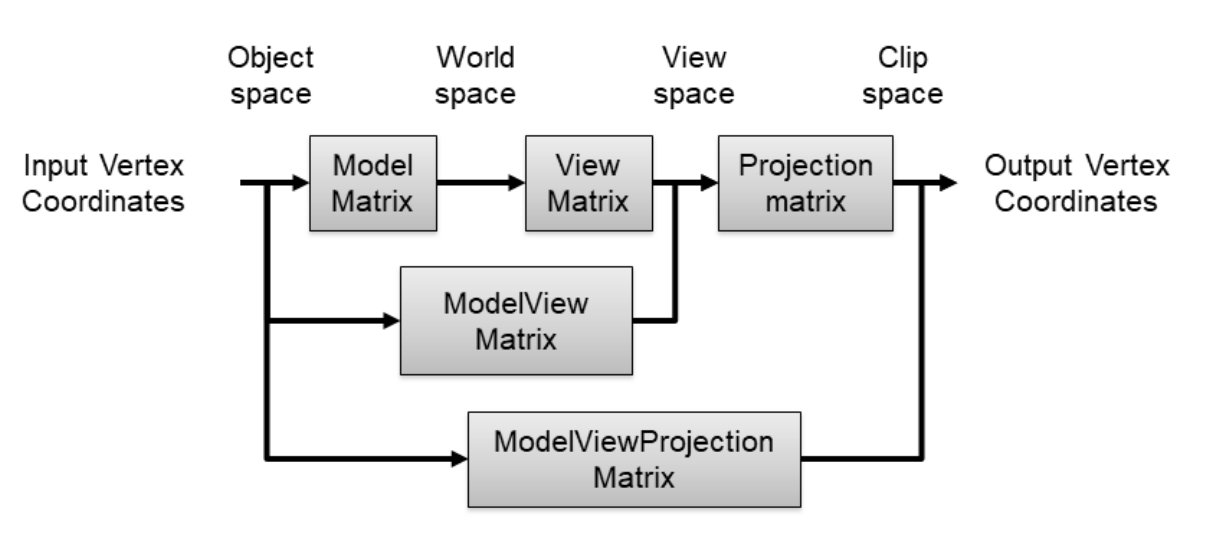
\includegraphics[scale=0.3]{inputvertextooutput}
\end{figure}

\subsubsection{Vertex Post-Processing}
This involves clipping, projection, and viewport transformation, which could be implemented to occur in any order.

\subsubsection{Geometry Shader}
This is an optional stage between the vertex shader and the fragment shader.

Unlike the vertex shader, the geometry shader has full knowledge of the primitive it is working on; it has access to each vertex of the primitive, including adjacency information.
It can also be used to generate primitives dynamically, such as in growing plants with procedural geometry.

\subsection{Rasterization Stage}
\begin{figure}[htb!]
  \centering
  \caption{The rasterization stage.}
  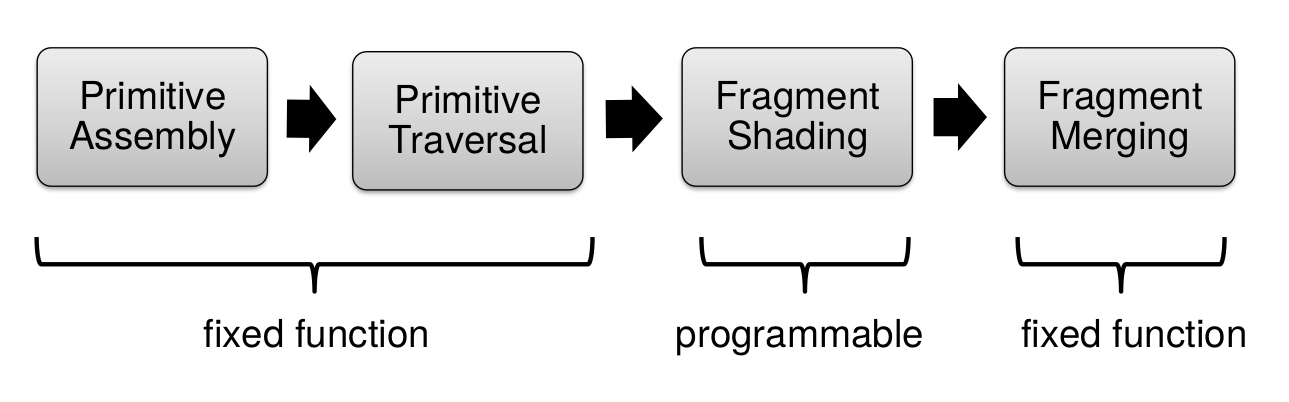
\includegraphics[scale=0.3]{rasterizationstage}
\end{figure}

Primitives are sampled into pixels on screen; discrete fragments are created from continuous surfaces.
The raster points are also called fragments; each fragment corresponds to one pixel in the frame buffer, and this corresponds to one pixel of the screen.

This involves:
\begin{itemize}
  \item \textbf{Primitive assembly} - backface culling and setup of the primitive for traversal.
  \item \textbf{Primitive traversal} (scan conversion) - sampling and interpolation of vertex attributes (e.g.\ depth, colour).
  \item \textbf{Fragment shading} - computing fragment colours based on textures, lighting calculations, etc.
  \item \textbf{Fragment merging} - composing the final pixel values from fragments over the same pixel; depth tests; blending\dots.
\end{itemize}

Different rules for rasterization are applied for each primitive type, this is called a \textit{fill convention}.

For polygons, we rasterize if the pixel centre is contained in the polygon, and if a pixel is on the edge, then only one is rasterized.

\subsection{Display Stage}
\begin{itemize}
  \item Gamma correction.
  \item Digital to analog conversion (historically).
  \item Digital scan-out, HDMI encryption, etc.
\end{itemize}

\subsubsection{Display Format}
The frame buffer pixel can be formatted as RGBA or as an index into a table of colours (obsolete).

\subsubsection{Functionality vs. Frequency}
\begin{itemize}
  \item \textbf{Geometry processing} (per-vertex):
    \begin{itemize}
      \item Transformation and lighting (T\&L).
      \item Historically floating point, complex operations.
      \item Millions of vertices per second.
      \item Today - \textbf{vertex shader}.
    \end{itemize}
  \item \textbf{Fragment processing} (per-fragment):
    \begin{itemize}
      \item Blending, texture combination.
      \item Historically fixed point and limited operations.
      \item Billions of fragments.
      \item Today - \textbf{fragment shader}.
    \end{itemize}
\end{itemize}

\subsection{Architectural Overview}
\begin{figure}[htb!]
  \centering
  \caption{Overview of the archiecture.}
  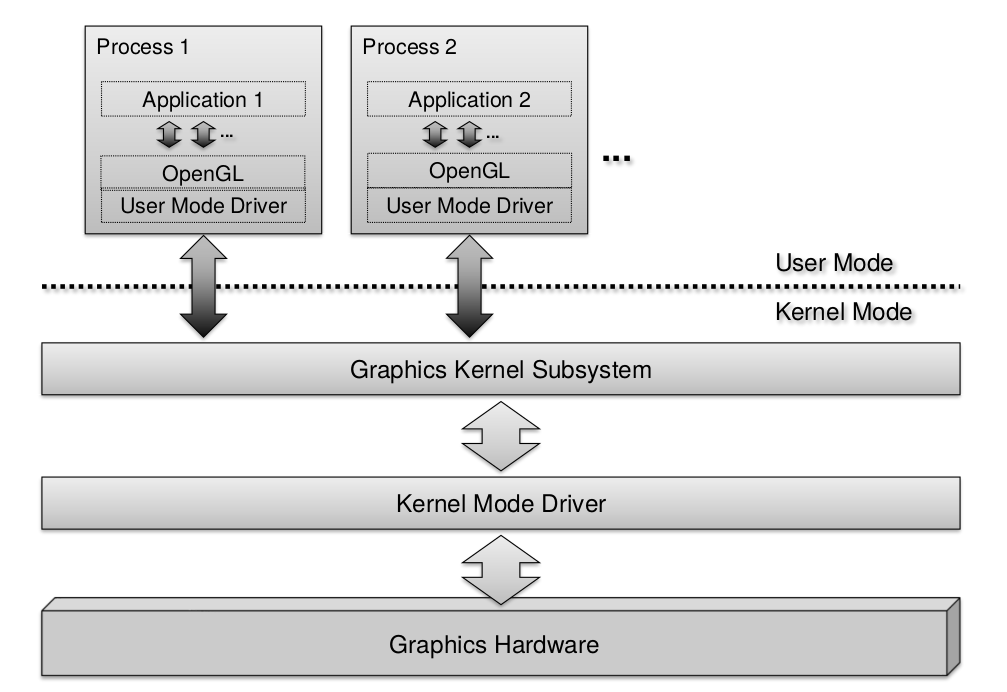
\includegraphics[scale=0.3]{architecture}
\end{figure}

\begin{itemize}
  \item The graphics hardware is a shared resource.
  \item \textbf{User Mode Driver} (UMD) - prepares command buffers for the hardware.
  \item \textbf{Graphics Kernel Subsystem} - schedules access to the hardware.
  \item \textbf{Kernel Model Drive} (KMD) - submits command buffers to the hardware.
\end{itemize}

\section{Graphics APIs}
\subsection{What is \textit{OpenGL}?}
\begin{itemize}
  \item Low-level graphics API specification.
    \begin{itemize}
      \item Interface is platform independent but the implementation is platform dependent.
      \item Defines an abstract rendering device and functions to operate it.
      \item Can draw, but no concept of permanent objects.
    \end{itemize}
  \item Platform provides the implementation, as part of the graphics driver or the runtime library on top of the driver.
  \item Initialization through platform specific API.
  \item State machine for high efficiency.
\end{itemize}

\subsection{\textit{GLSL}}
\textit{GLSL} is the shader language for \textit{OpenGL} and is used to define parts of the pipeline using own programs.
With the exception of rasterization, all processing steps of the graphics card can be programmed directly.

The application developer passes the shader source code and all additional variables and constants for each shader type to the \textit{OpenGL} driver.
The driver compiles and links the shaders to a shader program.

Each primitive sent by the application will pass through the shaders contained in the shader program in the following order:
\begin{enumerate}
  \item \textbf{Vertex Shader}:
    \begin{itemize}
      \item Executed once for each vertex.
      \item Shader only has access to vertex, but not neighbouring vertices or topology.
    \end{itemize}
  \item \textbf{Tessellation Shader}:
    \begin{itemize}
      \item An area (triangle or square) is divided into smaller areas.
    \end{itemize}
  \item \textbf{Geometry Shader}:
    \begin{itemize}
      \item Primitives can be created from an existing primitive (point, line, triangle).
    \end{itemize}
  \item \textbf{Fragment Shader}:
    \begin{itemize}
      \item Executed once for each fragment.
      \item The colour for the corresponding fragment is calculated.
    \end{itemize}
\end{enumerate}

\section{Illumination and Shading}
When we look at a point on an object, the colour and shading intensity perceived depend on various characteristics of the object and light sources that illuminate it.
\begin{itemize}
  \item \textbf{Object properties}:
    \begin{itemize}
      \item Position relative to the light sources.
      \item Surface normal vector.
      \item Albedo (ability to absorb light energy) of the surface, or reflectivity of the surface.
    \end{itemize}
  \item \textbf{Light source properties}:
    \begin{itemize}
      \item Intensity of emitted light.
      \item Distance to the point on the surface.
    \end{itemize}
\end{itemize}

\subsection{Radiometry}
\begin{defn}
  \textbf{Radiation flux} is the incident radiant energy over unit time.
\end{defn}

\begin{defn}
  \textbf{Radiance} is the radiant flux per unit solid angle per unit projected area.
  \[
    L(\omega) = \frac{d^2 \Phi}{\cos \theta dAd\omega} 
  \]
\end{defn}

\begin{defn}
  \textbf{Irradiance} is the differential flux falling onto differential area.
  \[
    E = \frac{d\Phi}{dA}
  \]
\end{defn}

\begin{defn}
  \textbf{Reflection} is the process by which electromagnetic flux incident on a surface leaves the surface without a change in frequency.
\end{defn}

\begin{defn}
  \textbf{Reflectance} is a fraction of the incident flux that is reflected.
\end{defn}

\subsection{Reflectance}
\begin{figure}[htb!]
  \centering
  \caption{Irradiance and radiance.}
  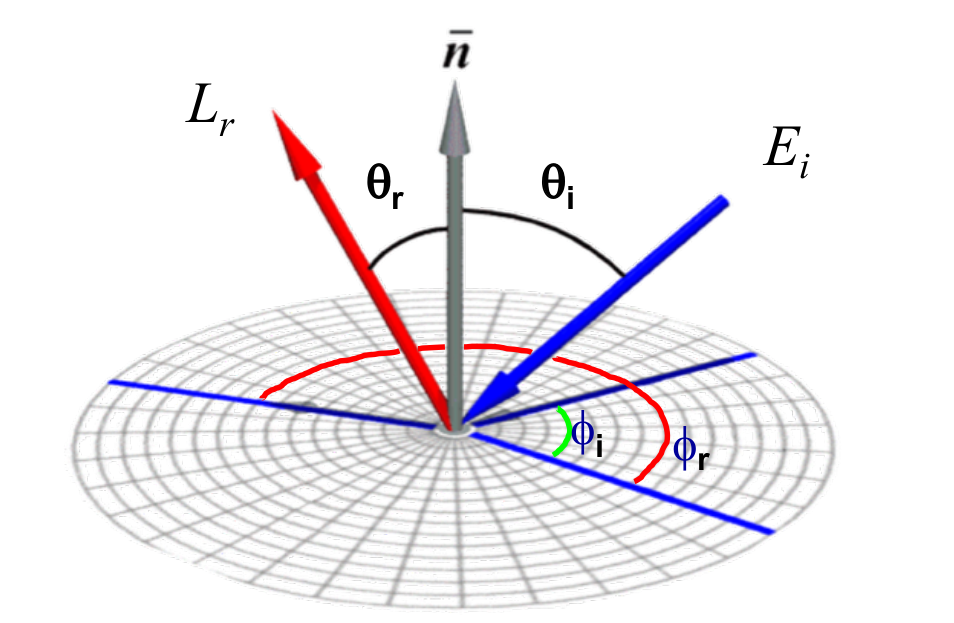
\includegraphics[scale=0.3]{brdf}
\end{figure}
\begin{defn}
  The \textbf{Bidirectional Reflectance Distribution Function} (BRDF) defines how light is reflected:
  \[
    f_r(\theta_i, \phi_i, \theta_r, \phi_r) = \frac{dL_r (\theta_r, \phi_r)}{dE_i (\theta_i, \phi_i)}  
  \]
\end{defn}

\subsubsection{Isotropic BRDFs}
Rotation along the surface normal does not change reflectance, so:
\[
  f_r(\theta_i, \phi_i, \theta_r - \phi_r) = f_r(\theta_i, \theta_r, \phi_d) = \frac{dL_r (\theta_r, \phi_d)}{dE_i (\theta_i, \phi_d)}  
\]

\subsubsection{Anisotropic BRDFs}
These are concerned with surfaces with strongly oriented microgeometry elements, e.g.\ brushed metals, hair, fur, cloth.

\subsubsection{Properties}
\begin{itemize}
  \item \textbf{Non-negativity}: $f_r(\theta_i, \phi_i, \theta_r, \phi_r) \geq 0$.
  \item \textbf{Energy Conservation}: $\int_\Omega f_r(\theta_i, \phi_i, \theta_r, \phi_r) d\mu(\theta_r, \phi_r) \leq 1 \text{ for all } (\theta_i, \phi_i)$.
  \item \textbf{Reciprocity}: $f_r(\theta_i, \phi_i, \theta_r, \phi_r) = f_r(\theta_r, \phi_r, \theta_i, \phi_i)$.
\end{itemize}

\subsubsection{BSSRDF}
The bidirectional scattering-surface distribution function is used with surfaces which have layers, e.g.\ skin.
Light may be absorbed by one layer and reflected by another.

\subsection{Ideal Diffuse Reflectance}
We assume the surface reflects equally in all directions, an ideal diffuse surface would be a very rough surface at the microscopic level, e.g.\ chalk, clay.

Then the value of the BRDF value would be constant throughout:
\[
  L_r(\omega_r) = \int_\Omega f_r(\omega_i, \omega_r) dE_i(\omega_i) = f_r \int_\Omega dE_i(\omega_i) = f_r E_i
\]

Ideal diffuse reflectors reflect light according to \textit{Lambert's cosine law} - this means that the greater the angle of the light direction to the surface normal (up to orthogonal), the less is reflected. 

We further model the reflectance as:
\[
  L(\omega_r) = k_d (\textbf{n} \cdot \textbf{l}) \frac{\Phi_s}{4\pi d^2} 
\]
where
\begin{itemize}
  \item $k_d$ is the diffuse reflection coefficient.
  \item $n$ is the surface normal.
  \item $l$ is the light direction.
\end{itemize}

We use $\max ((\textbf{n} \cdot \textbf{l}), 0)$ to avoid a negative dot product value when the vectors are facing away from each other, and must normalize the vectors before applying the dot product.

\subsection{Ideal Specular Reflectance}
Here, reflection is only at a mirror angle.
\begin{itemize}
  \item View dependent.
  \item Microscopic surface elements oriented in the same direction as the surface itself.
\end{itemize}

\begin{figure}[htb!]
  \centering
  \caption{Snell's Law.}
  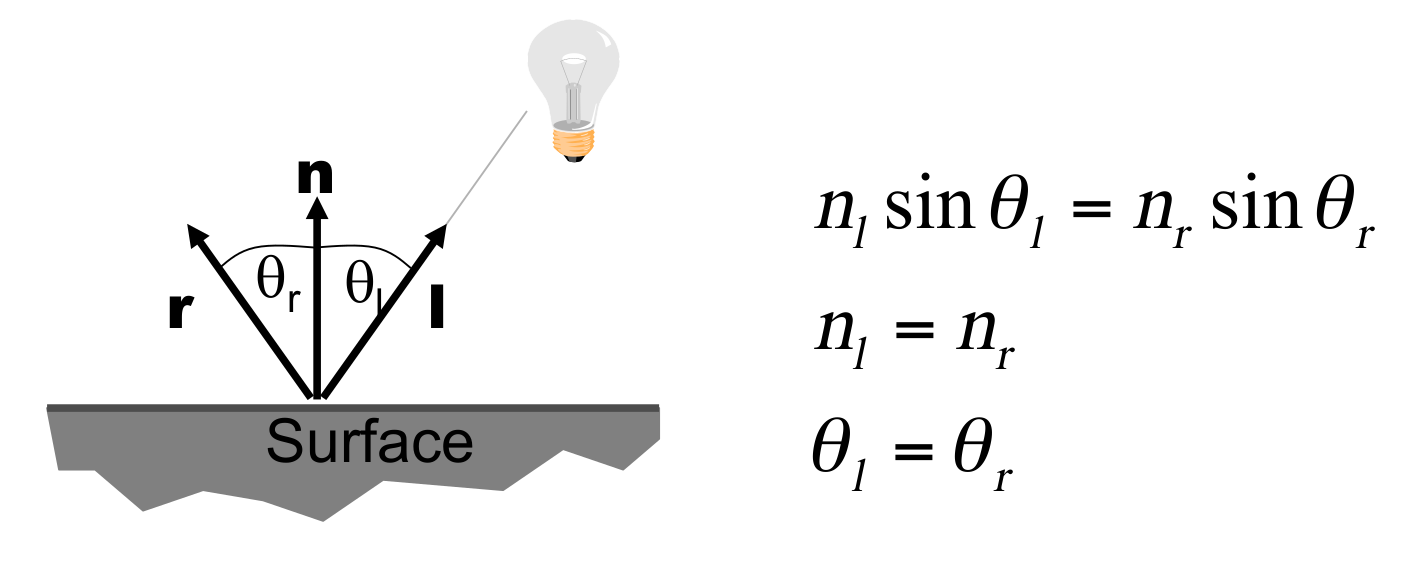
\includegraphics[scale=0.3]{snell}
\end{figure}

In \textit{Snell's Law}, the incoming ray, the surface normal, and the reflected ray all lie in a common plane.

\subsection{Non-Ideal Reflectors}
\textit{Snell's Law} only applies to ideal mirror reflectors, real materials tend to deviate significantly from ideal mirror reflectors and they are not ideal diffuse surfaces either.

\subsubsection{Simple Empirical Model}
\begin{itemize}
  \item Most of the reflected light travels in the direction of the ideal ray.
  \item We expect some to reflect slightly offset from the ideal.
  \item As we move further away in the angular sense from the reflected ray, less light is reflected.
\end{itemize}

\subsubsection{Surface Characteristics}
\begin{itemize}
  \item \textbf{Perfectly matte surface} - reflected intensity same in all directions.
  \item \textbf{Slightly specular (shiny) surface} - slightly higher intensity in the reflected direction.
  \item \textbf{Highly specular (shiny) surface} - high intensity in the reflected direction.
  \item \textbf{Perfect mirror} - all light is re-admitted in the reflected direction.
\end{itemize}

\subsection{Phong Model}

\begin{figure}[htb!]
  \centering
  \caption{The Phong model.}
  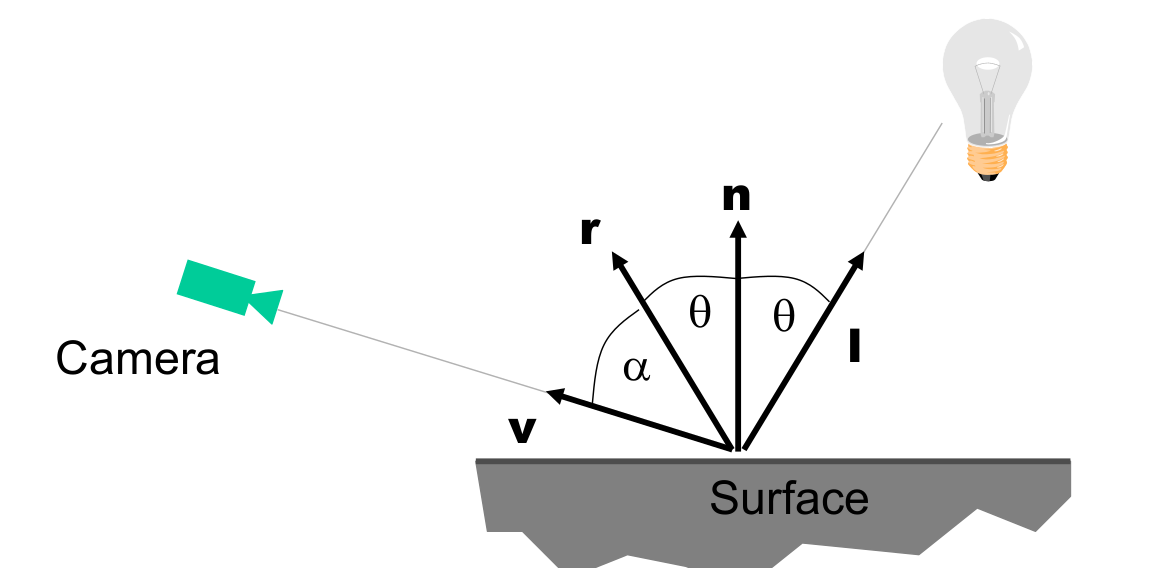
\includegraphics[scale=0.3]{phong}
\end{figure}
The light reflected depends on the angle between the ideal reflection direction and the viewer direction $\alpha$.

\[
  L(\omega_r) = k_s(\cos \alpha)^q \frac{\Phi_s}{4\pi d^2} = k_s (\textbf{v} \cdot \textbf{r})^q \frac{\Phi_s}{4\pi d^2} 
\]
where:
\begin{itemize}
  \item $k_s$ is the specular reflection coefficient.
  \item $q$ is the specular reflection exponent.
  \item $\textbf{r} = 2(\textbf{n} \cdot \textbf{l}) \textbf{n} - \textbf{l}$.
\end{itemize}

Higher values of $q$ result in greater, more centred reflections.

\subsubsection{Blinn-Phong Variation}
\begin{figure}[htb!]
  \centering
  \caption{The Blinn-Phong variation.}
  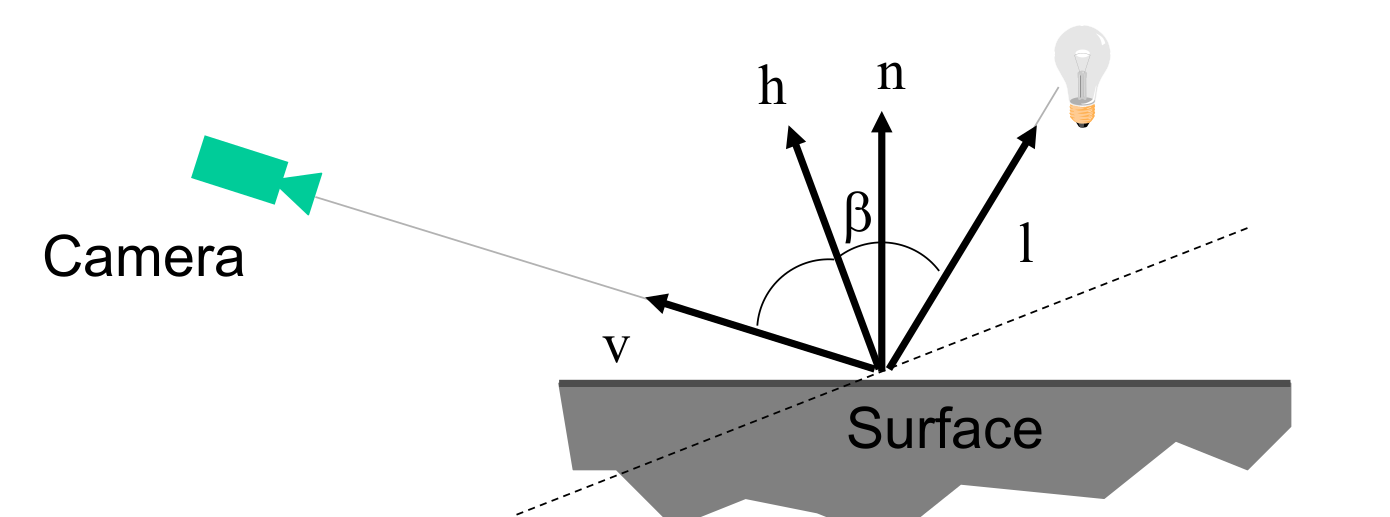
\includegraphics[scale=0.3]{blinnphong}
\end{figure}
We use the halfway vector $\textbf{h}$ between $\textbf{l}$ and $\textbf{v}$:
\[
  \textbf{h} = \frac{\textbf{l} + \textbf{v}}{\lVert \textbf{l} + \textbf{v} \rVert} 
\]
leading to:
\[
  L(\omega_r) = k_s(\cos \beta)^q \frac{\Phi_s}{4\pi d^2} = k_s (\textbf{n} \cdot \textbf{h})^q \frac{\Phi_s}{4\pi d^2} 
\]

\subsection{Ambient Illumination}
This represents the reflection of all indirect illumination - a hack.
\[
  L(\omega_r) = k_a 
\]
where $k_a$ is the ambient coefficient.

\subsection{Phong Illumination Model}
We sum up the three components, diffuse reflection + specular reflection + ambient:
\[
  L(\omega_r) = k_a + (k_d (\textbf{n} \cdot \textbf{l}) + k_s (\textbf{v} \cdot \textbf{r})^q) \frac{\Phi_s}{4\pi d^2} 
\]

\subsubsection{Inverse Square Law and Heuristic Law}
Since light falls off according to the inverse square law, we multiply by $\frac{\Phi_s}{4\pi d^2}$, where $d$ is the distance from the light source to the object.

Although this is physically correct, it does not produce the best results.
We often use $\frac{\Phi_s}{4\pi(d + s)}$, where $s$ is a heuristic constant.

\subsection{Shading}
There are three levels at which shading can be applied:
\begin{itemize}
  \item \textbf{Flat shading}.
  \item \textbf{Gouraud shading}.
  \item \textbf{Phong shading}.
\end{itemize}
where the latter are \textbf{interpolation shading}.

\subsubsection{Flat Shading}

\begin{itemize}
  \item Each polygon is shaded uniformly over its surface.
  \item Shade is computed by taking a point in the centre and the surface normal vector.
  \item Usually only defuse and ambient components used.
\end{itemize}

\subsubsection{Interpolation Shading}
\begin{figure}[htb!]
  \centering
  \caption{Calculating the shades at the edge.}
  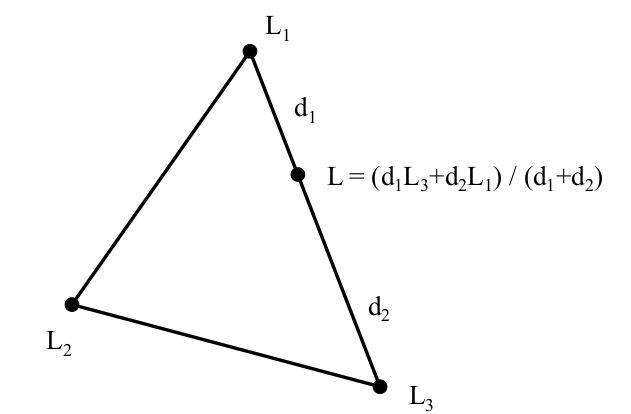
\includegraphics[scale=0.3]{interpolationedge}
\end{figure}

\begin{figure}[htb!]
  \centering
  \caption{Calculating the internal shades.}
  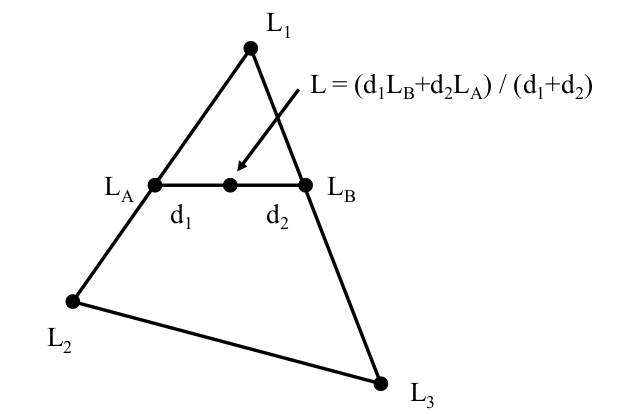
\includegraphics[scale=0.3]{interpolationinternal}
\end{figure}

\begin{itemize}
  \item Compute an independent shade value at each point.
  \item Done quickly by interpolation:
    \begin{enumerate}
      \item Compute a shade value at each vertex.
      \item Interpolate to find the shade value at the boundary.
      \item Interpolate to find the shade values in the middle.
    \end{enumerate}
\end{itemize}


\subsubsection{Interpolating over Polygons}
We can interpolate over groups of polygons to create the impression of a smooth surface.
The idea is to create at each vertex an averaged intensity from all the polygons that meet at that vertex.

To compute an average normal vector at a vertex:
\[
  n_ave = (n_1 + n_2 + n_3 + n_4) / 4
\]
where $n_i$ are the normal vectors of the polygons that meet at the vertex.

\subsubsection{Smooth Shading}
This requires per-vertex normals.
\begin{itemize}
  \item \textbf{Gouraud Shading}:
    \begin{itemize}
      \item Interpolate colour across triangles.
      \item Fast, supported by most graphics accelerator cards.
      \item Cannot model specular components accurately as we do not have the normal vector at each point on a polygon.
    \end{itemize}
  \item \textbf{Phong Shading}:
    \begin{itemize}
      \item Interpolate normals across triangles.
      \item More accurate specular modelling, but slower.
    \end{itemize}
\end{itemize}

\subsubsection{Interpolation of the 3D Normals}
We may express any point in parametric form:
\[
  \textbf{P} = \textbf{V}_1 + \mu_1 (\textbf{V}_2 - \textbf{V}_1) + \mu_2 (\textbf{V}_3 - \textbf{V}_1)
\]

The average normal vector at the same point may be calculated as the vector $\textbf{a}$:
\[
  \textbf{a} = \textbf{n}_1 + \mu_1 (\textbf{n}_2 - \textbf{n}_1) + \mu_2 (\textbf{n}_3 - \textbf{n}_1)  
\]
then:
\[
  \textbf{n}_{average} = \textbf{a} / \lvert \textbf{a} \rvert 
\]

Interpolation calculations may be done in either 2D or 3D, but for specular reflections the calculation of the reflected vector and viewpoint vector must be done in 3D.

\section{Colour}
Lasers are light sources that contain a single wavelength (or a narrow band of).
In practice, light is made up of a mixture of many wavelengths with an energy distribution.

Human colour vision is based on three cone cell types which respond to light energy in different bands of wavelength.
These bands overlap, which implies that colours do have a unique energy distribution.
Colours which are a distribution over all wavelengths can be matched by mixing three: \textbf{RGB}.

\subsection{Colour Matching}
Given any colour light source, we can try to match it with a mixture of three light sources:
\[
  X = rR + gG + bB 
\]
where $R, G, B$ are pure light sources, and $r, g, b$ are their intensities - for simplicity we drop $R, G, B$.

\subsection{Subtractive Matching}
Not all colours can be matched with a given set of light sources.
We can add light to the colour we are trying to match:
\[
  X + r = g + b 
\]

With this, we can match all colours.

\subsection{The CIE Diagram}
\begin{figure}[htb!]
  \centering
  \caption{CIE diagram.}
  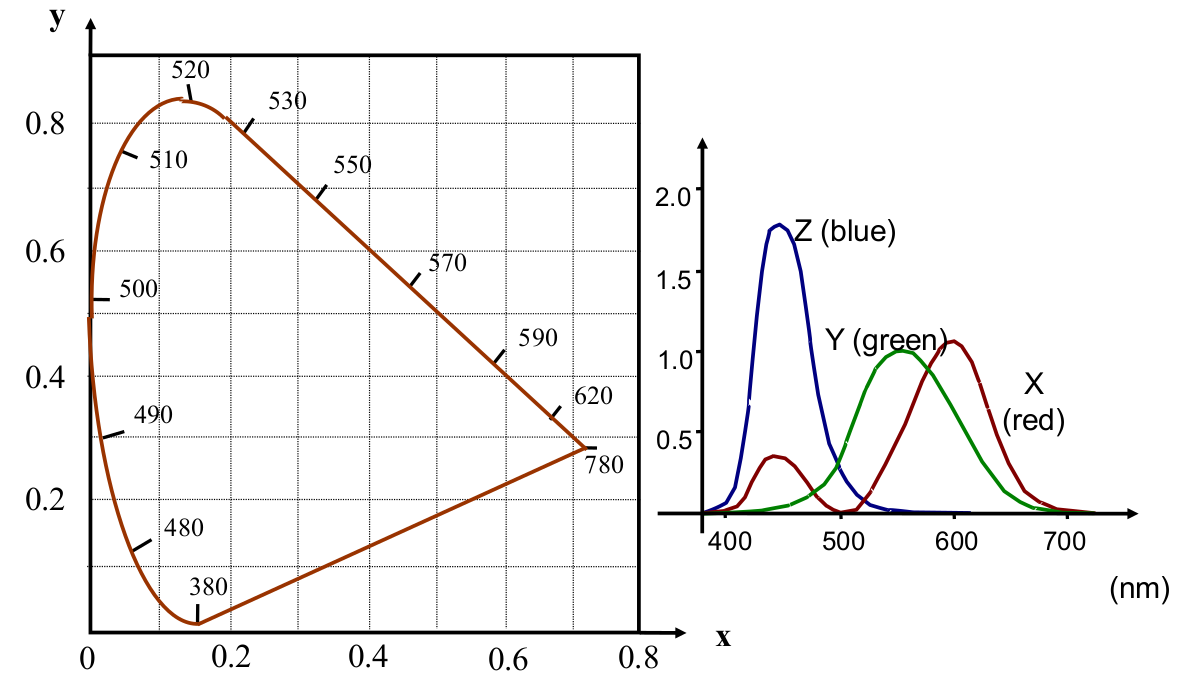
\includegraphics[scale=0.3]{cie}
\end{figure}
The CIE diagram is a standard normalised representation of colour.
Given three light sources, and allowing ourselves subtractive matching, we can mix them to match any given colour.

\subsubsection{Normalized Colours}
\begin{figure}[htb!]
  \centering
  \caption{Normalized colours.}
  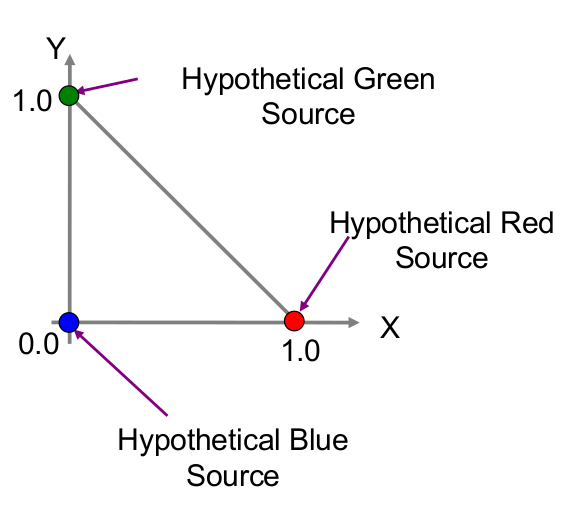
\includegraphics[scale=0.3]{normalizedcolours}
\end{figure}
We normalize the ranges found to $[0\dots1]$ to avoid the negative signs.
We then normalize the colours so that the three components sum to $1$:
\begin{align*}
  x &= r / (r + g + b) \\
  y &= g / (r + g + b) \\
  z &= b / (r + g + b) = 1 - x - y
\end{align*}

\subsubsection{Convex Shape}
The pure colours (coherent $\lambda$) are round the edge of the CIE diagram.
The shape must be convex (convex set) since any blend (interpolation) of pure colours should create a colour in the visible region.

Note that the line joining red and purple has no pure equivalent, the colours can only be created by blending.

\subsubsection{Intensities}
Since the colours are all normalized, there is no representation of intensity.
By changing intensity, different colours can be seen.

\subsubsection{White Point}
When the three components are equal, the colour is white.
This is seen at point $(0.33, 0.33)$.

\subsubsection{Saturation}
Pure colours are fully saturated, these correspond to the colours around the edge of the horseshoe.
Saturation of an arbitrary point is the ratio of its distance to the white point over the distance of the white point to the edge.

\subsubsection{Complement Colour}
THe complement of a fully saturated colour is the point diametrically opposite through the white point.
A colour added to its complement gives us white.

\begin{figure}[htb!]
  \centering
  \caption{Using the CIE diagram to find properties of a colour.}
  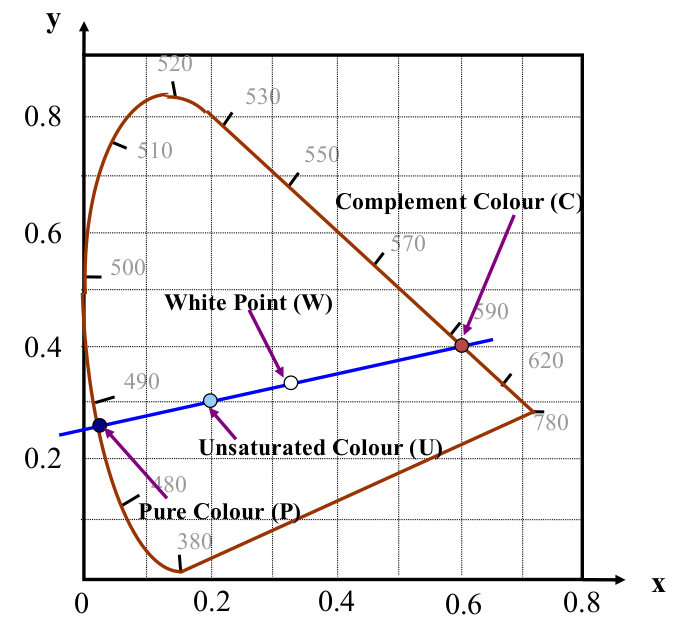
\includegraphics[scale=0.3]{cie2}
\end{figure}

\subsection{Subtractive Primaries}
When printing colour, we use a subtractive representation.
Inks absorb wavelengths from incident light so they subtract components to create colour.
The subtractive primaries are magenta, cyan, and yellow.

\subsection{Reproducible Colours}
Colour monitors are based on the output of three different light emitting phosphors or diodes.
The nominal position of these are:
\begin{center}
  \begin{tabular}{c c c c c}
    & x & y & z \\
    Red & 0.628 & 0.346 & 0.026 \\
    Green & 0.268 & 0.588 & 0.144 \\
    Blue & 0.150 & 0.07 & 0.780 
  \end{tabular}
\end{center}

The monitor RGB representation is related to CIE colours by:
\[
  (x, y, z) =
  \begin{pmatrix}
    0.628 & 0.268 & 0.15 \\
    0.346 & 0.588 & 0.07 \\
    0.026 & 0.144 & 0.78
  \end{pmatrix}
  \begin{pmatrix}
    R \\ G \\ B
  \end{pmatrix}
\]

\subsection{HSV Colour Representation}
RGB and CIE are practical representations and do not relate to how we perceive colours.
\begin{itemize}
  \item \textbf{Hue} - corresponds to pure colour.
  \item \textbf{Saturation} - proportion of pure colour.
  \item \textbf{Value} - the brightness (intensity).
\end{itemize}

\begin{align*}
  r = g &= b & H &\text{ is undefined} \\
  \min(r, g, b) &= b & H &= \frac{120(g - b)}{(r - b) + (g - b)} \\
  \min(r, g, b) &= r & H &= 120 + \frac{120(b - r)}{(g - r) + (b - r)} \\
  \min(r, g, b) &= g & H &= 240 + \frac{120(r - g)}{(r - g) + (b - g)}
\end{align*}

\[
  S = \frac{\max(r,g,b) - \min(r, g, b)}{\max(r, g, b)} 
\]

\[
  V = \max(r, g, b) 
\]

In the RGB system, each point is treated as a mixture of pure colour and white.
The smallest component is taken as white and the ratio of the other components (after subtraction of the white component) is the pure colour.

The pure colours however are not coherent wavelengths as in the CIE diagram.

\subsection{Alpha Channels}
The $\alpha$ value is the attenuation of the intensity, allowing greater flexibility in colour representation and avoids truncation errors at low intensity, or for masking certain parts of an image.
\begin{align*}
  \alpha &= 0 && \text{transparent} \\
  0 < \alpha &< 1 && \text{semi-transparent} \\
  \alpha &= 1 && \text{opaque}
\end{align*}

\[
  C = (R, G, B) \rightarrow C = (\alpha r, \alpha g, \alpha b, \alpha) 
\]

\end{document}
